\documentclass{article}

\usepackage[english]{babel}
\usepackage[margin=3cm]{geometry}
\usepackage{graphicx}
\usepackage{float}
\usepackage{caption}
\usepackage{hyperref}
\usepackage{amsmath}
\usepackage{wrapfig}
\usepackage[parfill]{parskip}

% fonts
\usepackage[T1]{fontenc}
\usepackage{helvet}
\renewcommand{\familydefault}{\sfdefault}

\graphicspath{{img/}}

% theorem environment
\usepackage{amssymb}

\newtheorem{theorem}{Definitie}[section]

\usepackage{enumitem}

\newenvironment{thmenum}
 {\begin{enumerate}[label=\upshape\bfseries(\roman*)]}
 {\end{enumerate}}


% code
\usepackage{minted}
\setminted{frame=single,framesep=3pt,linenos}
\usepackage{upquote}
\usepackage{color}

\begin{document}

\begin{titlepage}
    \author{Tuur Vanhoutte}
    \title{Linux OS}
\end{titlepage}

\pagenumbering{gobble}
\maketitle
\newpage
\tableofcontents
\newpage

\pagenumbering{arabic}

\section{Introductie}

\subsection{Verschil Server \& Workstation}

\subsubsection{Server}

\begin{itemize}
    \item Deliver services to (multiple) users
    \item Focussed: only this and nothing else
    \item Secure
    \item No GUI, everything happens through the commandline
    \item $\Rightarrow$ as small a footprint as possible
\end{itemize}

\subsubsection{Workstation}

\begin{itemize}
    \item Use services
    \item Create documents
    \item Look for information
    \item Consume multimedia
    \item GUI
    \item $\Rightarrow$ Large footprint
\end{itemize}

\subsection{Extra information/resources}

\begin{itemize}
    \item The Linux Documentation Project: \url{http://tldp.org}
    \item Pluralsight LPIC-1: Linux Professional Institute Certification: \url{https://www.pluralsight.com/paths/lpic-1}
    \item The Arch Linux Wiki is one of the most extensive sources of info about Linux: \url{https://wiki.archlinux.org}
    \begin{itemize}
        \item In this module we will use Debian, not Arch, but many things are very similar
    \end{itemize}
    \item Google
\end{itemize}

\subsection{What is Linux?}

\subsubsection{What is an operating system (OS)?}

\begin{theorem}[Operating System]
An operating system, or OS, is software that communicates with the hardware
and alows other programs to run. 

It is comprised of system software = the fundamental files your computer needs to function.
\end{theorem}


\textcolor{red}{Linux is NOT an operating system: Linux = the \underline{\textbf{kernel}}}

\subsubsection{What is a Kernel?}

\begin{theorem}[Kernel]
The kernel is software that is the core of a computer's operating system, with complete control over the system.

It is the first program loaded on start-up. 

It handles\dots: 

\begin{itemize}
    \item \dots the rest of the startup
    \item \dots input/output requests from software, translating them into instructions for the CPU
    \item \dots memory
    \item \dots peripherals
\end{itemize}
\end{theorem}


\subsection{GNU Operating System}

\begin{theorem}[GNU]
GNU = GNU's Not Unix (recursive acronym)

Founded by Richard Stallman (ex-MIT, founder of the Free Software Foundation), 1984

Goal: completely free Operating System
\end{theorem}

\subsection{Linux, the kernel}

By Linus Torvalds (Finland), 1991

\begin{itemize}
    \item Own personal development, not initially intended to distribute
    \item Interest from other developers, mainly to use with GNU OS
    \item Meanwhile contributions of over 12000+ developers
    \item 492 of top-500 supercomputers in the world run Linux
    \item Basis for Android, Chrome OS
\end{itemize}

Linux = the kernel

GNU = OS-tools around the kernel

$\Rightarrow$ \textbf{GNU/Linux}

\subsubsection{Distributions}

\begin{theorem}[Distribution]
A Linux distribution (or distro for short) is GNU/Linux + extra tools and applications to create a full-fledged OS.

That distribution can be easily copied and installed to other computers.
\end{theorem}

\begin{itemize}
    \item RedHat (CentOS)
    \item Debian (Ubuntu)
    \item Arch Linux
    \item Void Linux
    \item Gentoo
    \item Pop! OS
\end{itemize}

\begin{figure}[H]
    \centering
    \includegraphics[width=0.75\textwidth]{redhat-vs-debian-tree.png}
    \caption{\url{https://upload.wikimedia.org/wikipedia/commons/1/1b/Linux_Distribution_Timeline.svg}}
\end{figure}

\url{https://en.wikipedia.org/wiki/List_of_Linux_distributions}

\subsection{Open Source}

\begin{theorem}[Open Source]
Open source software is software of which the code is licensed to be open to everyone. 

Anyone can use, change, distribute the software. This allows code to be developed in a public manner.
\end{theorem}

\textbf{\textcolor{red}{OPEN SOURCE DOES NOT MEAN FREE}}

\subsubsection{Commercial distributions}

= Open source, non-free distributions

\begin{itemize}
    \item SUSE Linux Enterprise Server (SLES)
    \item SUSE Linux Enterprise Desktop (SLED)
    \item Red Hat Enterprise Linux (RHEL)
    \item Oracle Enterprise Linux
\end{itemize}

Commercial distributions have official support channels.

$\Rightarrow$ You're not paying for the operating system, you're paying for the support.

\subsubsection{In this course: Debian}


\begin{itemize}
    \item Current version: 10.7
    \item Forms the basis of many others: Ubuntu, Raspbian, Knoppix, Linux Mint
    \item Available on many platforms: Intel x86, AMD64, Intel64, ARM, MIPS, Power Systems, \dots
\end{itemize}

\section{Debian Installation}

\textbf{See Labs for detailed Installation tutorial}

\subsection{Networking in Linux (with VMWare)}

\begin{itemize}
    \item VMWare presents ethernet adapter
    \item During creation of virtual machine: MAC-address is created
    \item During installation: network configuration through DHCP
    \begin{itemize}
        \item IPv4-address
        \item Default gateway
        \item DNS-server
        \item \underline{Optional:} proxy-server
    \end{itemize}
\end{itemize}

\subsection{Users in Linux}

\begin{itemize}
    \item Linux is multi-user from the ground up
    \begin{itemize}
        \item Multiple users can be active at the same time
    \end{itemize}
    \item `Administrator'-user is called root
    \item Each user has a user-ID (uid)
    \begin{itemize}
        \item root has uid=0
        \item uid=0 has all rights
    \end{itemize}
    \item Each user has a home-directory
\end{itemize}

\subsection{Disks, partition, filesystems}

\begin{itemize}
    \item Our VM has 1 disk
    \begin{itemize}
        \item Presented on the SCSI-bus
        \item First disk on SCSI-bus: \textbf{sda}
        \item Then sdb, sdc, \dots
    \end{itemize}
    \item Disk = concatenation of blocks
    \item Divide blocks in collections (=partitions)
    \begin{itemize}
        \item 1st partition: sda1
        \item 2nd partition: sda2
        \item \dots
    \end{itemize}
    \item 2 types of partitions
    \begin{itemize}
        \item Primary
        \item Extended
    \end{itemize}
\end{itemize}

\subsubsection{Partitions}

Primary partition

\begin{itemize}
    \item A filesystem can be created inside this
    \item Up to 4 primary partitions
\end{itemize}

Extended Partition

\begin{itemize}
    \item `Logical' partitions can be created inside this
\end{itemize}

Our setup:

\begin{itemize}
    \item sda1: primary partition
    \item sda2: extended partition
    \item sda5: `logical' partition inside extended partition sda2
\end{itemize}

\begin{figure}[H]
    \centering
    \includegraphics[width=0.3\textwidth]{partitions.png}
    \caption{Our setup}
\end{figure}

\subsection{Partitioning schemes}

= a set of rules describing how a disk should be partitioned.
A disk partitioning scheme is chosen by desired flexibility, speed, security, and necessary disk space.

\subsubsection{MBR}

We use the MBR Partitioning scheme

\begin{theorem}[MBR]
MBR, or Master Boot Record, is a special type of boot sector at the start of a disk.

It contains: 

\begin{itemize}
    \item a set of instructions necessary to boot operating systems.
    \item info about how partitions are placed on disk
\end{itemize}


\end{theorem}

\textbf{Limitations:}

\begin{itemize}
    \item Maximum disks of 2TB
    \begin{itemize}
        \item 32-bit for number of logical sectors
        \item Common sector size: 512 bytes
        \item $2^{32} \cdot 512\ \text{bytes} = 4294967296 \cdot 512\ \text{bytes} \approx 2\text{TB}$
    \end{itemize}
    \item Maximum amount of primary partitions = 4
\end{itemize}

BIOS can boot from a disk with MBR partitioning

\subsubsection{GPT}

\begin{theorem}[GPT]
GPT, or GUID Partition Table, is a standard for the layout of partition tables on a disk.
It's an alternative to MBR.

It uses unique identifiers (GUIDs) 
\end{theorem}

\begin{itemize}
    \item BIOS cannot boot from a disk with GPT-partitioning: UEFI required when using GPT
    \item GPT allows disks larger than 2TB
\end{itemize}

\begin{theorem}[UEFI]
UEFI, or Unified Extensible Firmware Interface, is a newer firmware interface by Intel (90's) that replaces the BIOS interface by IBM (70's).
\end{theorem}

\textbf{How does it work?}

\begin{itemize}
    \item Disk = collection of blocks
    \item Group of blocks together = sector
    \item Common sector size: 512 bytes
    \item Sectors indicated with Logical Block Addresses (LBA)
    \item MBR in LBA 0
    \item GPT headers in LBA 1
    \item Partition tabel right after that
\end{itemize}




\subsubsection{Bootstrap procedure}

\begin{enumerate}
    \item Motherboard gets electricity
    \item Mini-loader hardcoded in memory
    \begin{itemize}
        \item BIOS gets loaded
    \end{itemize}
    \item Boot media are consulted
    \item First boot medium, first sectors are being read $\Rightarrow$
    \item MBR contains a bit-more-advanced loader: GRUB
    \begin{itemize}
        \item \underline{GR}and \underline{U}nified \underline{B}ootloader
    \end{itemize}
    \item This loader loads a more advanced loader (GRUB second stage bootloader)
    \item The OS is loaded
\end{enumerate}

\subsubsection{Linux boot process}

6 high level steps

\begin{itemize}
    \item BIOS (Basic Input/Output System) - loads MBR
    \item MBR (Master Boot Record) - loads GRUB
    \item GRUB (Grand Unified Bootloader) - loads kernel
    \item Kernel - executes /sbin/init
    \item Init - executes runlevel programs
    \item Runlevel - programs from /etc/rc.d/rcXX.d are started
\end{itemize}

\subsubsection{BIOS <> UEFI}

\begin{itemize}
    \item Recent systems use UEFI, not BIOS
    \item UEFI is required to boot from GPT-disk
    \item Linux has no trouble working with UEFI
\end{itemize}

\textbf{So why will we use MBR?}

\begin{itemize}
    \item Virtualisation is the norm
    \item Virtual machines typically have small disks
    \item Small disks are MBR partitioned
\end{itemize}



\subsection{Filesystems}

\subsubsection{Windows}

\begin{itemize}
    \item FAT (1977)
    \item FAT32 (1996)
    \item NTFS (1993)
    \item ReFS (2012)
\end{itemize}

\subsubsection{Linux}

\begin{itemize}
    \item Ext (1992)
    \item Ext2 (1993)
    \item Ext3 (2001)
    \item Ext4 (2008)
    \item ZFS (2005)
    \item BtrFS (2007)
\end{itemize}

\subsubsection{Swap}

= Paging

\begin{itemize}
    \item Free up physical memory (RAM) by moving pages to slower storage (storage disks instead of RAM)
    \item Page out $=$ memory page moves to swap
    \item "Swapiness"
    \begin{itemize}
        \item = parameter between 0 and 100
        \item = how quickly linux will swap
        \begin{itemize}
            \item 0 = very conservative
            \item 100 = very agressive
        \end{itemize}
    \end{itemize}
    \item Windows uses a swap file (pagefile.sys)
    \item Linux uses a swap partition
\end{itemize}

\subsection{File structure}



\begin{figure}[H]
    \centering
    \includegraphics[width=0.4\textwidth]{linux-filestructure.png}
    \caption{Linux uses a tree structure}
\end{figure}

\begin{figure}[H]
    \centering
    \includegraphics[width=0.5\textwidth]{windows-filestructure.png}
    \caption{Windows uses a similar structure, but every volume uses a letter.}
\end{figure}

\begin{figure}[H]
    \centering
    \includegraphics[width=0.5\textwidth]{linux-filestructure2.png}
    \caption{With linux, volumes are `mounted' to folders somewhere under root /}
\end{figure}

\subsection{Configuration}

\subsubsection{Packages}

\begin{itemize}
    \item Tools and applications are build up by files
    \item All files belonging to 1 application are bundled in a package
    \item Packages in debian have the .deb extension
\end{itemize}

Repositories

\begin{itemize}
    \item Packages are collected in repositories
    \item Are made available through the internet
    \item Packages have dependencies
\end{itemize}

\subsubsection{Package management}

Debian: dpkg \& apt (Advanced Package Tool)

\begin{itemize}
    \item dpkg: Install, remove, give info about .deb packages
    \begin{itemize}
        \item dpkg -l = lists packages 
    \end{itemize}
    \item apt: Get packages from a repository and install, remove, give info, ...
    \begin{itemize}
        \item apt update
        \begin{itemize}
            \item Contact the repositories
            \item Get most recent list of packages and versions
        \end{itemize}
        \item apt upgrade
        \begin{itemize}
            \item Of the packages which are more recent in the repositories compared to what is installed: install newest version
        \end{itemize}
        \item apt install <xyz>
        \begin{itemize}
            \item Download package <xyz> from the repository
            \item Check the dependencies and download depending packages
            \item Install package <xyz> and all corresponding dependencies
        \end{itemize}
    \end{itemize}
\end{itemize}

Which repositories? See /etc/apt/sources.list for the list of repositories. You can add/remove/change repositories in this file.

\subsubsection{Useful packages}

\begin{itemize}
    \item open-vm-tools
    \item vim
    \item sudo
    \item tcpdump
\end{itemize}

Install multiple pacakges in one command: apt install vim sudo tcpdump ntp

\subsection{Shutdown of VM}

\begin{itemize}
    \item Power button (=ACPI shutdown)
    \item Shut down operating system only
    \begin{itemize}
        \item = halt
    \end{itemize}
    \item Shut down operating system and VM, multiple ways:
    \begin{itemize}
        \item shutdown -P now
        \item init 0
        \item poweroff
    \end{itemize}
    \item Reboot
    \begin{itemize}
        \item reboot
        \item init 6
        \item shutdown -r now
    \end{itemize}
\end{itemize}

\subsection{Basic network}

\begin{itemize}
    \item No GUI $\Rightarrow$
    \item Layer 1: Physical (VMWare virtual network)
    \item Layer 2: Datalink (Ethernet \& MAC address)
    \item Layer 3: Network (IPv4)
    \item Layer 4: Transport (Transport Control Protocol (TCP), User Datagram Protocol (UDP))
    \item Layer 5: Application (SSH, HTTP, \dots)
\end{itemize}

\subsubsection{Basic networking commands}

\begin{itemize}
    \item arp
    \item ping
    \item route
    \item bmon
\end{itemize}

\subsection{Services}

\begin{itemize}
    \item Processes that `listen' on the network
    \begin{itemize}
        \item TCP or UDP port
    \end{itemize}
    \item Overview of currently running / listening services: ss command
    \begin{itemize}
        \item ss -tulpn
        \item t: show TCP
        \item u: show UDP
        \item l: show listening
        \item p: show process ID
        \item n: no name-resolving
    \end{itemize} 
\end{itemize}

\subsection{Wooclap Questions}

\begin{itemize}
    \item Why do we talk about GNU/Linux?
    \item What is a kernel?
    \item What is the difference between Open Source and free?
    \item How is the Administrator user called? What is its uid?
    \item What is MBR?
    \item What are the limitations of MBR? (Solution?)
    \item What is swap? What is swappiness?
    \item What is a package?
    \item What is a repository?
    \item What is a dependency?
    \item What is a package manager?
    \item What is the difference between 'apt update' and 'apt upgrade'
    \item Which protocol makes the link between MAC address \& IP address?
    \item Which command gives you the current ARP-table?
    \item What are the 5 layers of the TCP/IP network model?
    \item How do you find the MAC-address of a network interface?
    \item Put Linux boot process in correct order (6 levels)
    \item What is a linux distribution?
\end{itemize}

\section{File structure}

\begin{itemize}
    \item Tree structure
    \begin{itemize}
        \item Leaves = files
        \item Branches = directories
        \item The tree is inverted, root = /
    \end{itemize}
    \item Everything is a file (even devices, random numbers, and RAM) under 1 root
    \item This is in contrast to Windows, where every volume is a root.
\end{itemize}

\begin{figure}[H]
    \centering
    \includegraphics[width=0.4\textwidth]{linux-filestructure.png}
\end{figure}



\subsection{Intermezzo: single user mode}

\begin{itemize}
    \item Linux (the kernel) is built up as a multi-user system from the beginning
    \item Standard behaviour = multi-user
    \item But: also possible to boot in single-user mode
    \begin{itemize}
        \item No daemons, no multiple logins
        \item Sometimes called \textbf{Maintenance mode}
    \end{itemize}
    \item Examples of usage
    \begin{itemize}
        \item Filesystem repairs
        \item Upgrade of distribution
        \item Password recovery
        \item Adjustments to the root filesystem
        \item Forensics after security incident
    \end{itemize}
\end{itemize}

\subsubsection{Runlevels}

= predefined operating system status

\begin{itemize}
    \item Is presented with a number
    \item Linux has 7 runlevels:
    \begin{itemize}
        \item 0 = system halt (= VM shutdown)
        \item 1 = single user
        \item 2 = multi-user, no NFS (no network services, not often used)
        \item 3 = multi-user, CLI (Command Line Interface)
        \item 4 = self-definable
        \item 5 = multi-user, GUI (Graphical User Interface, if installed)
        \item 6 = reboot
    \end{itemize}
\end{itemize}

\subsection{Intermezzo: Add disk}

\textbf{Add a new disk without shutting down the system}

\begin{enumerate}
    \item Adjust VM: add disk
    \item Detect added disk
    \item Partition disk
    \begin{itemize}
        \item fdisk (for MBR)
        \item parted (for GPT)
    \end{itemize}
    \item Create filesystem
    \begin{itemize}
        \item Partition = collection of blocks (sectors)
        \item Not usable for the OS $\Rightarrow$ create filesystem
        \item mkfs.ext4 /dev/sdb1
        \begin{figure}[H]
            \centering
            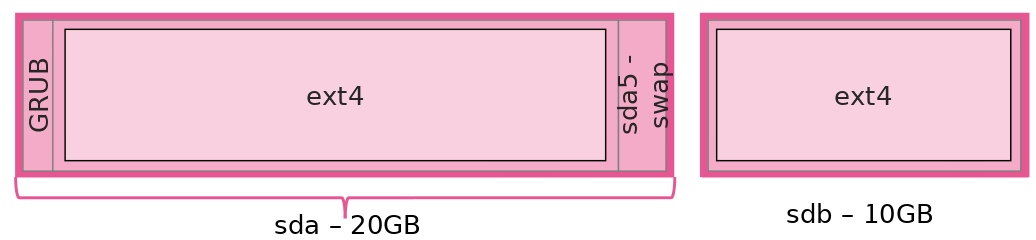
\includegraphics[width=0.7\textwidth]{create-filesystem.png}
        \end{figure}
    \end{itemize}
    \item Mount filesystem
    \begin{itemize}
        \item mkdir /mnt/datadisk
        \item mount /dev/sdb1 /mnt/datadisk
        \item see if it worked: df -h
    \end{itemize}
\end{enumerate}

\textbf{For detailed steps: see labs!}


\subsubsection{What after a reboot?}

Use /etc/fstab = a file that contains what needs to be mounted at boot

\begin{itemize}
    \item Device (/dev/sdXY or UUID) 
    \item Mountpoint (/mnt/folder)
    \item Type of filesystem (ext4, ntfs, \dots)
    \item Options
\end{itemize}


\subsection{Navigate through the tree}

\begin{itemize}
    \item pwd
    \begin{itemize}
        \item Print working directory
        \item Shows where in the tree you are
    \end{itemize}
    \item ls
    \begin{itemize}
        \item Show a list of files in the working directory
        \item ls -la : 10 characters at the beginning of each line. The d == directory (see later)
    \end{itemize}
    \item When you login, you are in your home directory
    \item / (= the filesystem root) is not the same as /root (the home directory of the root user)
    \item . = current directory
    \item .. = the directory one higher
\end{itemize}

\subsubsection{Relative vs absolute path}

Relative paths:

\begin{itemize}
    \item cd .. = go to the directory above the current directory
    \item cat ../etc/issue = go to the etc directory, one directory above the current directory. Open the issue file
\end{itemize}

Absolute paths:

\begin{itemize}
    \item cd / = go to the root directory
    \item cat /etc/issue = go to the etc/ directory under / (root)
\end{itemize}

\subsection{Filesystem Hierarchy Standard (FHS)}

\begin{itemize}
    \item Describes how the filesystem in Linux is build up
    \item Maintained by the Linux Foundation
    \item Most recent version: v3.0 (2015)
\end{itemize}



\subsubsection{Rules in the standard}

\begin{itemize}
    \item / is the root of the tree structure
    \item /bin 
    \begin{itemize}
        \item essential binaries (executable files), required for single user mode
    \end{itemize}
    \item /boot
    \begin{itemize}
        \item the place on the filesystem where the boot files reside
        \item configuration files for GRUB
        \item kernels
        \item initrd
        \begin{itemize}
            \item initial RamDisk
            \item During boot a temporary root-filesystem is being created in RAM
            \item This is used so the kernel can load important modules, so it can then switch to the real root filesystem
            \item part of step 3 of the linux boot process (BIOS - MBR - GRUB - kernel - init - runlevel)
        \end{itemize}
    \end{itemize}
    \item /dev
    \begin{itemize}
        \item Devices get a place in the filesystem
        \begin{itemize}
            \item sda
            \item rtc
            \item random
            \item cpu
            \item urandom
            \item null
        \end{itemize}
        \item ls -lah /dev/
    \end{itemize}
    \item /etc
    \begin{itemize}
        \item Host-specific sytem-wide configuration files
        \item Configuration for this host, readable for the whole system
    \end{itemize}
    \item /home
    \begin{itemize}
        \item Each (non-system) user has a home directory
        \item except for root $\Rightarrow$ /root
    \end{itemize}
    \item /mnt
    \begin{itemize}
        \item (temporarily) `mounted' filesystems
        \begin{itemize}
            \item Network shares
            \item USB-disk
            \item DVD-ROM
            \item Extra disks
        \end{itemize}
        \item Some distributions use /media for this
    \end{itemize}
    \begin{figure}[H]
        \centering
        \includegraphics[width=0.3\textwidth]{linux-filestructure2.png}
    \end{figure}
    
    \item /opt
    \begin{itemize}
        \item Optional application software packages
        \item Our installation $\Rightarrow$ no applications installed yet = empty (for now)
    \end{itemize}
    \item /proc
    \begin{itemize}
        \item Virtual filesystem
        \item Provides information about processes and the linux kernel
        \item cat /proc/cpuinfo
        \item cat /proc/sys/net/ipv4/ip\_forward
        \item cat /proc/partitions
    \end{itemize}
    \item /sbin
    \begin{itemize}
        \item Essential system binaries
        \item Only executable by root user
        \item fsck, init, route
    \end{itemize}
    \item /tmp
    \begin{itemize}
        \item Directory for temporary files
        \item Emptied at reboot (with most distributions)
    \end{itemize}
    \item /usr
    \begin{itemize}
        \item Read-only user data
        \item Constains most user (non-root) utilities and applications
    \end{itemize}
    \item /var
    \begin{itemize}
        \item Variable files
        \item Files that are expected to change continuously during normal system use
        \item Logs, spool files, temporary e-mail files, \dots
    \end{itemize}
\end{itemize}

\subsection{Some useful tips}

\subsubsection{History}

\begin{minted}{bash}
~# history

# shows a list of former commands executed by this user
# spans log-in sessions
# in reality, it shows the contents of the ~/.bash_history file
# if you use another shell like zsh, it's the ~/.zsh_history file
\end{minted}

CTRL + r:

\begin{itemize}
    \item Search the command history
    \item Show commands that match what you're typing
    \item repeatedly press ctrl+r to scroll through results
\end{itemize}


\subsubsection{Bind mount}

\textbf{Situation}

\begin{itemize}
    \item /mnt/storage is the normal mountpoint for other filesystems (e.g. SAN)
    \item Filesystem could not be mounted, but a process already started writing data
    \item $\Rightarrow$ this data arrives on the / filesystem under the directory /mnt/storage
    \item Problem fixed and filesystem can be mounted again $\Rightarrow$ mounted under /mnt/storage
    \item $\Rightarrow$ the already written data is now hidden
\end{itemize}

\textbf{The solution}

\begin{itemize}
    \item Create /mnt/storage and put some data in it
    \item Create a 1GB disk, ext4 formatted, mount under /mnt/storage $\Rightarrow$ data is now hidden
    \item Use mount -o bind to get data back without unmounting
\end{itemize}

\subsubsection{dd}

= Command to read or write bytes

\begin{minted}{bash}
# Example: overwrite first 2048 bytes of a disk with zeros
~# dd if=/dev/zero of=/dev/sdb count=4 bs=512
# Example: overwrite disk with random data when taking out of service
~# dd if=/dev/random of=/dev/sdb bs=1M
\end{minted}

\subsection{Wooclap Questions}

\begin{itemize}
    \item How do you ask the shell in which folder you are currently in?
    \item What is meant with the term 'runlevel' in Linux
    \item Describe single user mode with 1 word when you think of its primary use
    \item What is / are the most common runlevel(s) under linux? (So not all of them!)
    \item Where can you find the devices under Linux?
    \item What is the home directory of the root user?
    \item What command do we use to create a filesystem in a partition?
    \item What file do you need to edit to have a mounted filesystem available even after reboot?
    \item Where can you put temporary files in a linux system?
    \item How can you quickly search through your previously used commands?
    \item How do you quickly search through previously typed commands?
    \item What is swap?
    \item What are the limitations of MBR?
    \item What can you use a bind mount for?
\end{itemize}

\section{Filesystems}

\subsection{Introduction}

Books:

\begin{itemize}
    \item A group of letters together = a word
    \item A group of words together = a sentence
    \item A group of sentences together = a book
    \item A collection of books together = a library
    \item Books are ordered/sorted according to a certain system
    \begin{itemize}
        \item Best known: Dewey Decimal System
    \end{itemize}
\end{itemize}

Computers: 

\begin{itemize}
    \item Work with 0's and 1's
    \item 1 character in ASCII or ISO-8859-1 = 8bits (1 byte)
    \item 1 Unicode character in UTF-8: between 8 and 32 bits (4 bytes)
    \item Gets stored on block devices
    \begin{itemize}
        \item Hard devices, SSDs, RAMdisk, USB-stick
        \item The opposite of block devices = character devices 
    \end{itemize}
    \item System needs to organize this
\end{itemize}

\subsection{Blocks}

\begin{itemize}
    \item Disk = blocks
    \item Collection of blocks = sector (mostly 512 bytes)
    \item Collection of sectors = partition
    \item Partition not usable for an OS $\Rightarrow$ filesystem needed
\end{itemize}

\begin{theorem}[Filesystem]
    A filesystem is the methods and data structures that an operating system uses to keep track of files on a disk or partition; that is, the way the files are organized on the disk.
\end{theorem}

Several choices:

\begin{itemize}
    \item Ext2/3/4
    \item BrtFS
    \item ZFS
    \item \dots
\end{itemize}

\subsection{ext2/3/4}

Ext3 and Ext4 have journaling:

\subsubsection{Journaling}

\begin{itemize}
    \item Keeping track of changes that have not been committed to disk in a sort of 'diary'
    \item A kind of logbook of previous actions
    \item Why?
    \begin{itemize}
        \item Bring filesystem online faster after system crash or power failure
    \end{itemize}
\end{itemize}

\subsection{RAID}

\begin{theorem}[RAID]
    Redundant Array of Independant Disks (RAID) is a data storage virtualisation technology that combines multiple physical disk drive into one ore more logical units.

    Many purposes:

    \begin{itemize}
        \item Data redundancy
        \item Performance Improvement
        \item Both
    \end{itemize}
\end{theorem}

\subsubsection{RAID Controller}

\begin{itemize}
    \item Disks are connected to the controller
    \item The RAID controller displays the disks as 1 disk to the OS
    \item Nowadays, we call the RAID Controller the Host Bus Adapter (HBA)
    \item 
\end{itemize}

\subsubsection{RAID 0}

RAID level 0 uses striping:

\begin{theorem}[Striping]
    Data striping is the technique of segmenting logically sequential data (files) so that segments are stored on different physical storage devices

    Purpose:

    \begin{itemize}
        \item Increasing data throughput
        \item Balancing I/O load accross an array of disks
    \end{itemize}
\end{theorem}

\begin{figure}[H]
    \centering
    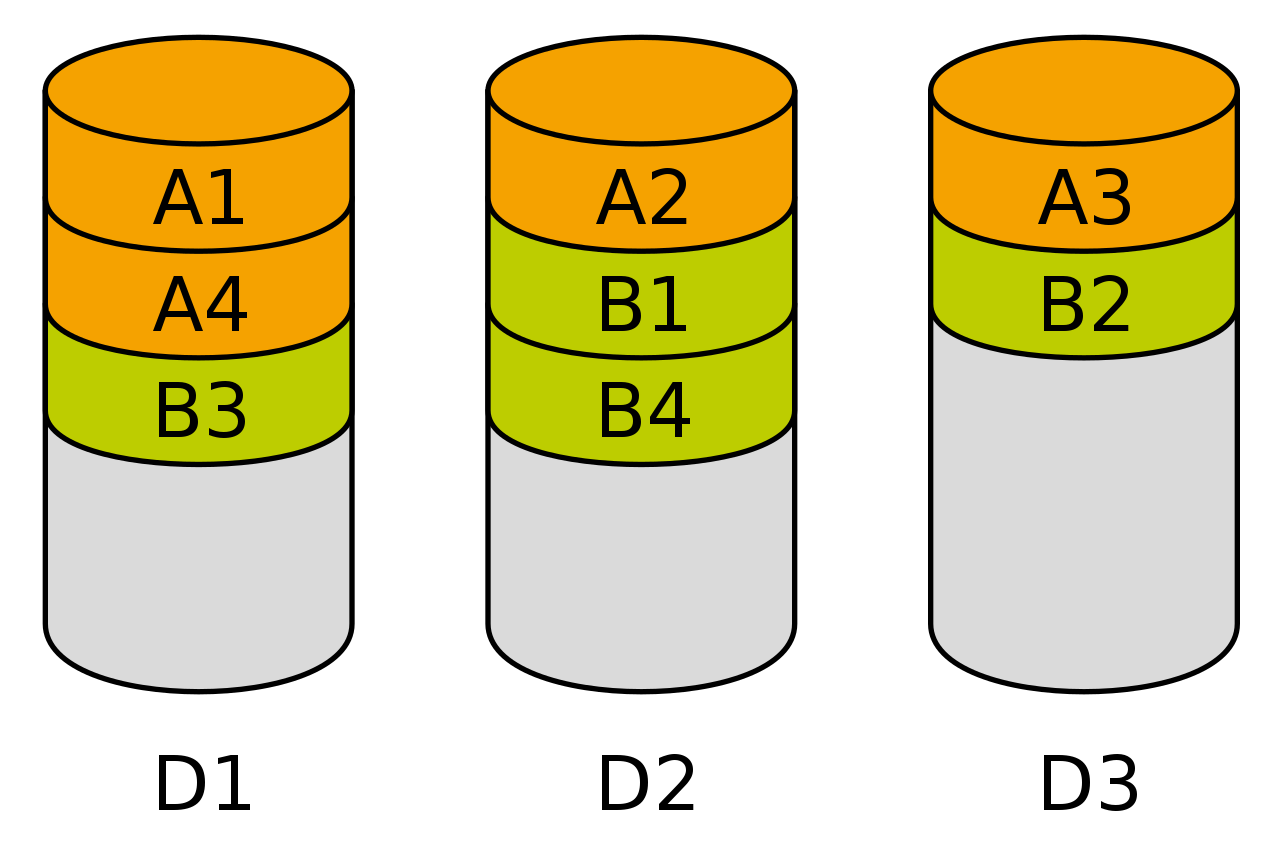
\includegraphics[width=0.3\textwidth]{raid-striping.png}
    \caption{Example: files A and B (4 blocks each) are spread over disks D1-D3}
\end{figure}


\subsubsection{RAID 1}

RAID level 1 uses mirroring:

\begin{theorem}[Mirroring]
    Disk mirroring is the replication of logical disk volumes onto seperate physical disks.

    Purpose:

    \begin{itemize}
        \item Continuous availability: in case of hardware failure, you always have a backup of your data
        \item Increasing read speeds
    \end{itemize}
\end{theorem}

\begin{figure}[H]
    \centering
    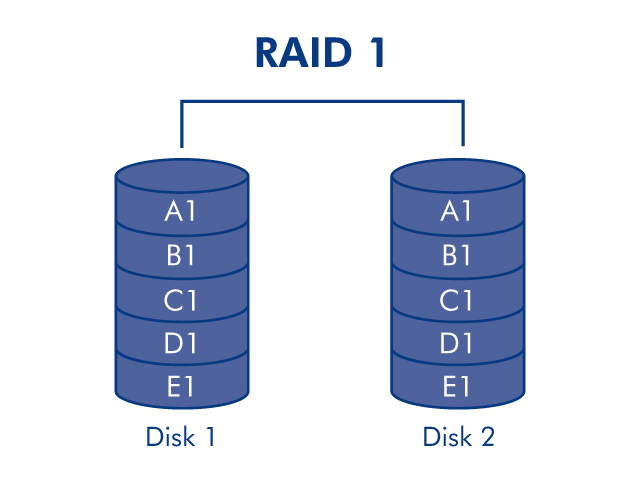
\includegraphics[width=0.3\textwidth]{raid-mirroring.png}
    \caption{RAID 1}
\end{figure}


\subsubsection{RAID 4}

\begin{itemize}
    \item If we have at least 3 disks
    \item For every block of data:
    \begin{itemize}
        \item Divide the block in 2 halves: A and B
        \item Write A to disk 1
        \item Write B to disk 2
        \item Write A+B to disk 3
    \end{itemize}
    \item $\Rightarrow$ RAID 4 is striping (disk 1 \& 2) with parity (disk 3)
    \item Capacity x2
    \item Read speed x2
    \item Write speed is limited, because of the need to write all parity data to a single disk
\end{itemize}

\begin{figure}[H]
    \centering
    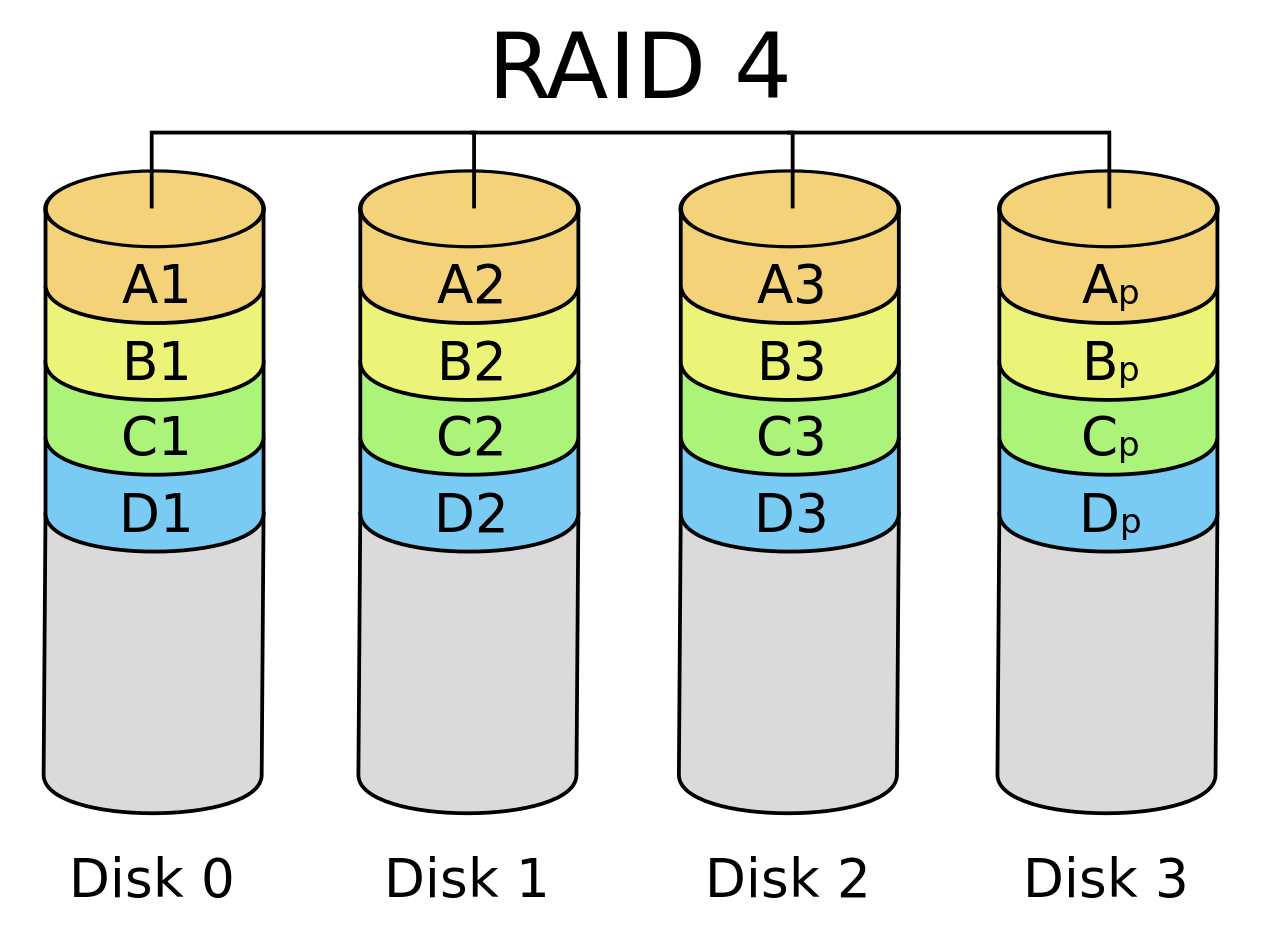
\includegraphics[width=0.3\textwidth]{raid-4.png}
    \caption{A RAID-4 setup with 4 disks. Disk 3 is the parity disk}
\end{figure}


\subsubsection{RAID 5}

RAID level 5 like RAID 4, but the parity is distributed.

\begin{itemize}
    \item This evens out the stress of a dedicated parity disk (RAID 4)
    \item Write performance is increased
\end{itemize}

\begin{figure}[H]
    \centering
    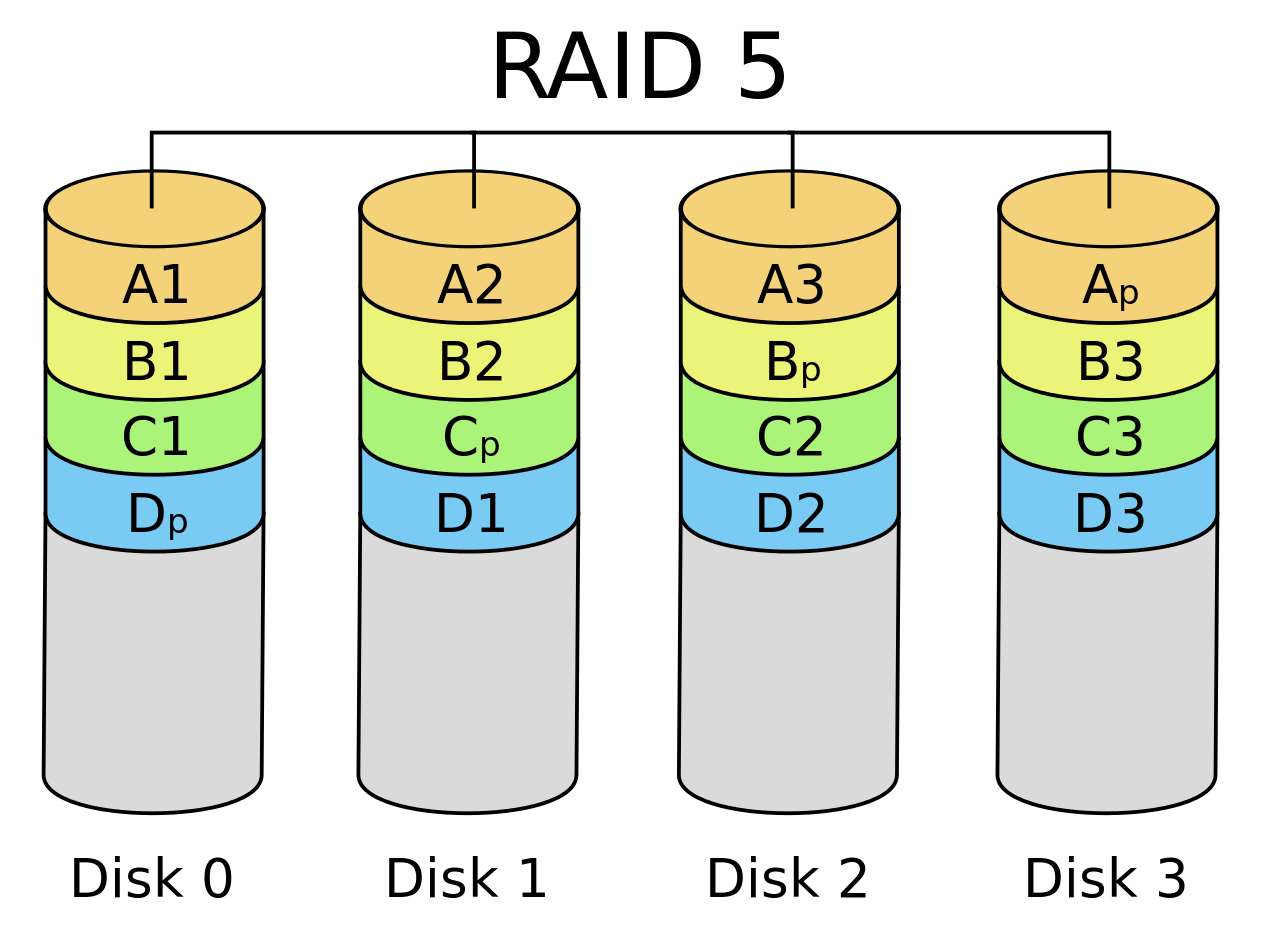
\includegraphics[width=0.3\textwidth]{raid-5.png}
    \caption{RAID-5: distributed parity with 4 disks}
\end{figure}


\subsubsection{RAID 6}

RAID level 6 like RAID 5, but with a second parity block.

\begin{figure}[H]
    \centering
    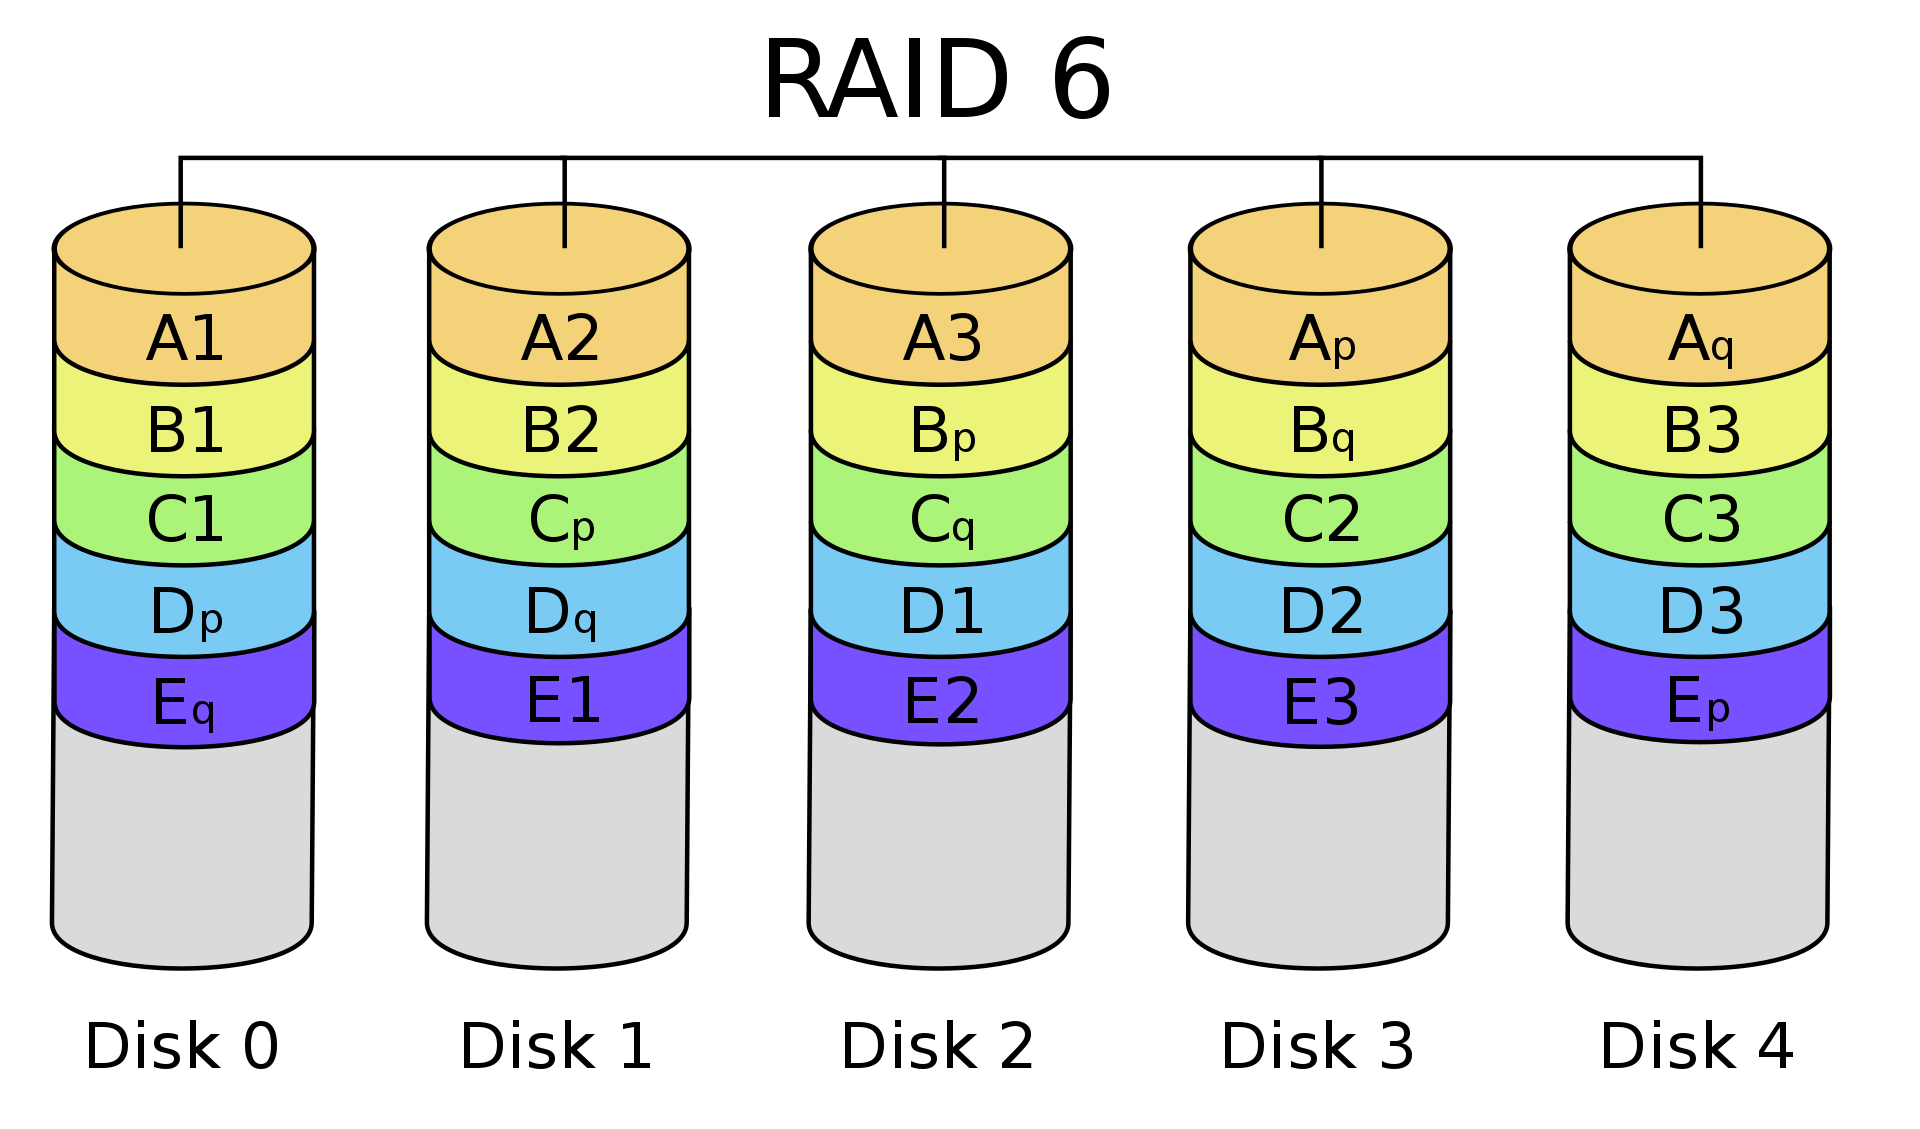
\includegraphics[width=0.3\textwidth]{raid-6.png}
\end{figure}



\subsubsection{Disk failure}

For every RAID level, a certain amount of disks can fail without it becoming a problem:

\begin{itemize}
    \item RAID 0: no disks can fail: if any disk fails, you lose data
    \item RAID 1: Every disk except for one can fail
    \item RAID 5: 1 disk can fail
    \item RAID 6: 2 disks can fail
\end{itemize}

\subsubsection{Compound RAID levels}

Combining RAID levels is possible:

\begin{itemize}
    \item RAID 10 = RAID 1 + RAID 0
    \item RAID 01 = RAID 0 + RAID 1
    \item RAID 50 = RAID 5 + RAID 0
\end{itemize}

\subsection{OpenZFS}

\subsubsection{ZFS}

\begin{itemize}
    \item Zettabyte File System
    \item Developed by Sun (2011) $\Rightarrow$ Open source
    \item Now Oracle (2010) $\Rightarrow$ Not free and closed source
\end{itemize}

\subsubsection{Open ZFS}

\begin{itemize}
    \item Fork van ZFS
    \item 2013
    \item Option in Ubuntu-installer
\end{itemize}

Features:

\begin{itemize}
    \item Long term storage
    \item Checksum of all data and metadata
    \item Native RAID levels (0, 1, 5, 6, \dots)
    \item All data gets written through Copy-On-Write:
    \begin{itemize}
        \item COW = when a write request is made, the data is copied into a new storage area, and then the original data is modified.
        \item Redirect-on-write or ROW: the original storage is never modified. When a write request is made, it is redirected away from the original data into a new storage area.
    \end{itemize}
    \item Snapshots (read-only and mountable)
    \item Transparent compression
    \item Huge storage possibilities: up to 256 quadrillion zettabytes
    \item 128 bits system
\end{itemize}

\subsection{Intermezzo: Kernel modules}

\begin{itemize}
    \item Linux = kernel
    \item Kernel = modular
    \item /boot/config-4.9.0-13-amd64: config for this kernel
    \begin{itemize}
        \item Describes what is inside this kernel
    \end{itemize}
    \item Not all modules are loaded all the time
\end{itemize}

\subsubsection{Commands}

\begin{minted}{bash}
# Request current list of modules:
~# lsmod

# Load module:
~# modprobe brtfs

# Remove module ("unload"):
~# rmmode brtfs

\end{minted}

\subsection{Intermezzo: Snapshots}

\begin{itemize}
    \item Literally: a photograph of your filesystem
    \item Captures a the state of the filesystem at a certain point in time
    \item "The possibility to return in time"
\end{itemize}

\subsubsection{Do we still need backups if we have snapshots?}

YES!

\begin{itemize}
    \item RAID 1 (mirroring) only protects against disk failure, nothing else
    \item If someone deletes all data from one disk, the RAID controller will delete all data from the other disk.
    \item Snapshots can get lost: what if your server fails?
    \item $\Rightarrow$ backups can be stored safely, on other disks
\end{itemize}

\section{File manipulation}

\subsection{Basics}

\begin{minted}{bash}
# create an empty file called 'test'
~$ touch test

# edit a file
~$ vim test

# remove file
~$ rm rabbot

# move the file to /tmp
~$ mv test /tmp/

# rename the file
~$ mv test rabbit

# Linux doesn't really look at file extensions
# check the file extension:
~$ file <filename>
~$ file /boot/inird.img-4.9.0-13-amdb64
~$ file /etc/init.d/networking
\end{minted}

\subsection{Bundle files}

\begin{itemize}
    \item Tape ARchiver: TAR
    \begin{itemize}
        \item Created originally to bundle files/directories for storage on tapes
    \end{itemize}
    \item You can combine tar with gzip: .tar.gz
    \begin{itemize}
        \item tar cfv bundle.tar *.txt $\Rightarrow$ not compressed
        \item tar czfv bundle.tar.gz $\Rightarrow$ compressed
    \end{itemize}
\end{itemize}

\begin{minted}{bash}
~$ mkdir bundle
~$ cd bundle
~$ touch 1.txt 2.txt 3.txt
~$ tar cfv bundle.tar *.txt
# c = create a new archive
# f = specify a filename (bundle.tar)
# v = verbose: show what happens
~$ tar --list -f bundle.tar
~$ file bundle.tar

# extracting
~$ tar zxvf bundle.tar.gz
# z = zipped (compressed)
# x = eXtract
# v = verbose
# f = the argument (a file) 
\end{minted}

\subsection{Links and inodes}

\begin{itemize}
    \item Modern filesytems support links
    \item This is different from shortcuts in Windows:
    \item Windows shortcuts are text files that refer to other files
\end{itemize}

\subsubsection{Inodes}

\begin{theorem}[Inode]
    An inode is a data structure on a filesystem on Unix-like operating systems that 
    stores all the information about a file except its name and its actual data

    Metadata: data about the file
    \begin{itemize}
        \item Creation date
        \item Creation author
        \item Access rights
        \item \dots
    \end{itemize}
\end{theorem}

\subsubsection{Symbolic links}

\begin{theorem}
    A symbolic link (also symlink or soft link) is a term for any file that contains a reference to another file or directory in the form of an absolute or relative path

    Also called 'softlinks'
\end{theorem}

\begin{minted}{bash}
~$ ln -s <target> <link-name>
~$ ln -s /etc/issue test-link
# try out the following commands after creating a link:
~$ cat test-link
~$ file test-link
~$ cat /etc/issue
\end{minted}


\subsubsection{Hardlinks}

\begin{itemize}
    \item Same file, different name
    \item A hardlink refers to an inode, while a softlink refers to a file (which refers to an inode)
\end{itemize}

\begin{figure}[H]
    \centering
    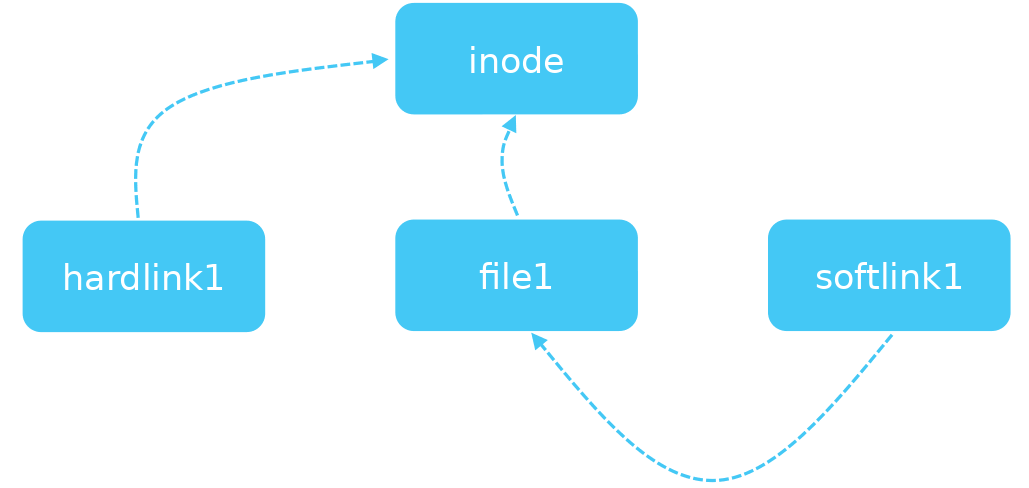
\includegraphics[width=0.5\textwidth]{soft-vs-hard-links.png}
    \caption{Symlink vs Hardlink}
\end{figure}


\subsection{File permissions}

\begin{figure}[H]
    \centering
    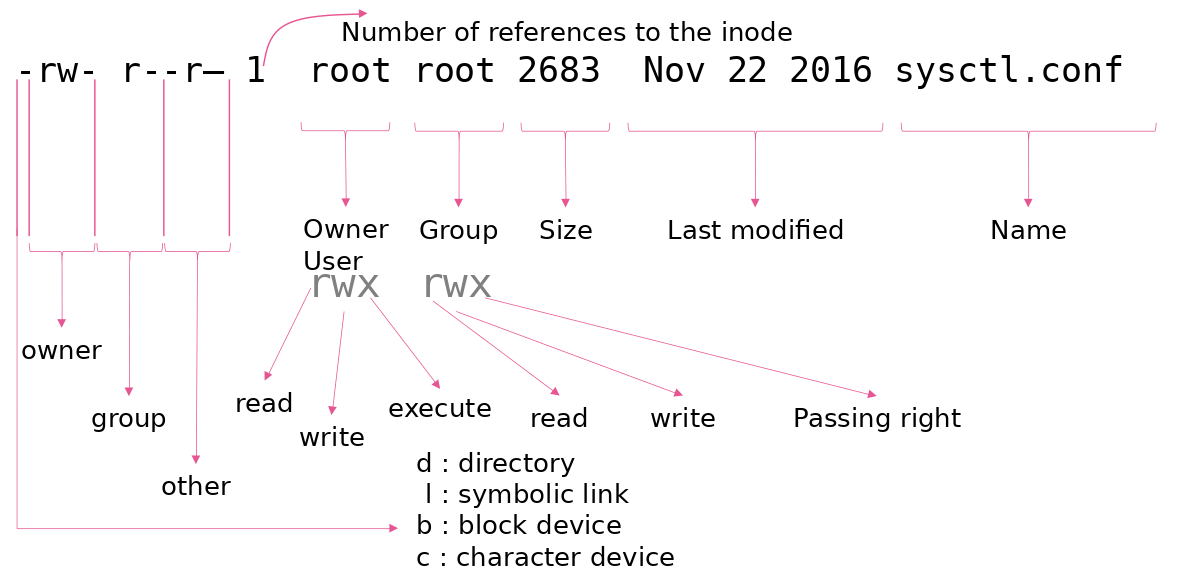
\includegraphics[width=0.8\textwidth]{file-permissions.png}
    \caption{The output of `ls -l' creates this type of output}
\end{figure}

\begin{enumerate}
    \item first character: type of file (directory, symbolic link, block device, character device)
    \item next 9 characters: owner rights, group rights, other rights
    \item next number: number of references to the inode
    \item owner user
    \item owner group
    \item size of file
    \item last modified
    \item name of file
\end{enumerate}

\begin{minted}{bash}
    # change the owner and group of a file or directory
    ~# chown <user>:<group> <file>
    ~# chown root:staff file.txt
    
    # change the rights for a file
    # chmod: change mode
\end{minted}

\begin{figure}[H]
    \centering
    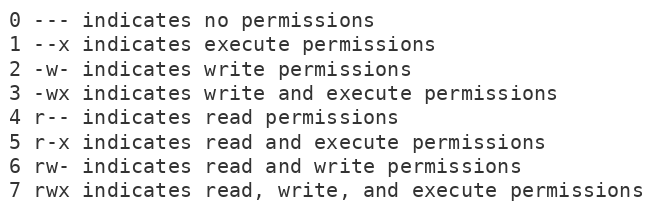
\includegraphics[width=0.5\textwidth]{octal-notation.png}
    \caption{Octal notation}
\end{figure}


\subsection{Overview of basic commands}

Usage and details for these commands: see labs

\begin{itemize}
    \item cat: print contents of file to terminal
    \item cut: cut (structured) input on a specific place: show a certain column, etc\dots
    \item grep: display lines for which the pattern matches
    \item egrep: extended grep, better handling of regular expressions
    \item find: search for files in a hierarchy of files and directories
    \item head: show first lines of file
    \item tail: show last lines of file
    \item less: show the contents of a text file, interactively
    \item man: show manual page for specific command
    \item wc: word count (but also character count, byte counts, newline counts, \dots) for a file
    \item date: show or configure system date and time
    \item cal: show a textual calendar
    \item sort: sort a file
    \item uniq: in a sorted output: count double lines or only show unique lines
\end{itemize}

\subsection{Wooclap}

\begin{itemize}
    \item What is meant by the term journaling for filesystems?
    \item Why is journaling used with filesystems?
    \item Give 2 examples of filesystems under linux that use journaling.
    \item How can you find out which kernel modules are currently loaded?
    \item Which command can you use to load a kernel module? 
    \item And which to 'unload' a kernel module?
    \item How many disks do you need at least to build a RAID10 system? Why?
    \item What is meant by a 'Copy On Write' filesystem?
    \item What are the advantages of a CoW filesystem?
    \item What are snapshots (in the context of storage systems)?
    \item What are the disadvantages of a CoW filesystem?
    \item Why do you still need backup when you have RAID1 and have snapshots?
    \item How can you find out which 'type' is a file? There are no extensions.
    \item What is an inode?
    \item What is the difference between a softlink and a hard link?
    \item At the output of the command ls -la: Which values can the first character of the line have and what do they mean?
    \item At the output of the command ls -la: Which possible values can the 3 groups of 3 characters have to describe the rights?
    \item With what command can you 'change' the 'owner' of a file or directory?
    \item With which command can you 'change' the rights of a file or directory?
    \item What does number 5 mean when you use it to determine file system permissions?
    \item What does number 7 mean when you use that to determine file system rights? Explain why.
    \item Which command do you use to cut structured input at a specific location?
    \item Which command do you use to display the first 16 lines of a text file?
    \item Which command can you use to find out all the modified files from the last 24 hours?
    \item Which command do you use to display the last 12 lines of a text file?
    \item How can you find out how long it has been since a linux system was rebooted?
    \item Which command can you use to get an overview of all daemons that are currently active in your system?
\end{itemize}

\section{Text editors, Piping, Redirection \& Jobs}

\subsection{Text editors}

\begin{itemize}
    \item Emacs (productivity, extensibility)
    \item Nano (simplicity)
    \item Vi / Vim (=VI iMproved) (productivity)
    \item Ne
\end{itemize}

Our choice: Vim

\subsubsection{vi vs vi-improved}

\begin{itemize}
    \item Navigating in vi: HJKL (left, down, up, right)
    \item Navigating in vim: HJKL or arrow keys
\end{itemize}

\begin{figure}[H]
    \centering
    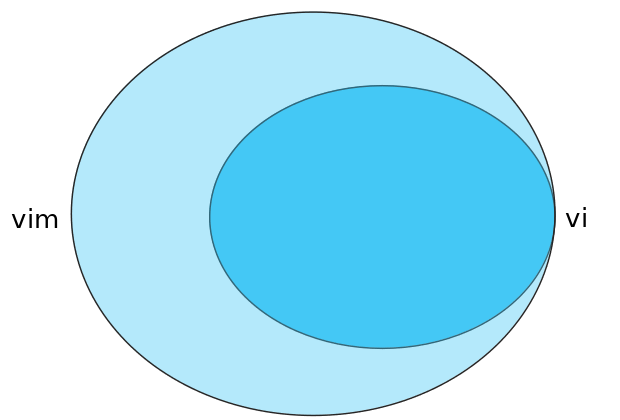
\includegraphics[width=0.5\textwidth]{vi-vim.png}
    \caption{Everything you can do in vi, you can do in vim, and more!}
\end{figure}

\subsubsection{First steps in vim}

\begin{minted}{bash}
# start vim:
$~ vim

# start vim tutorial:
$~ vimtutor
\end{minted}

\begin{itemize}
    \item bottom left of window: the current mode
    \item INSERT = the mode that lets you enter text
    \item Enter INSERT mode: i
    \item Leave INSERT mode and go to normal mode: ESC
    \item Once in normal mode, you can enter commands using `:'
    \item ESC : q $\Rightarrow$ quit
    \item ESC : w $\Rightarrow$ quit
    \item ESC : wq $\Rightarrow$ write and quit
\end{itemize}

\begin{minted}{bash}
# copy a line of text
ESC
# put cursor on the line you want to copy
yy # yank yank: copy a line of text
p # put: paste the copied line

# copy 2 lines of text and paste it 8 times:
ESC 2yy # 2 yank yank: yank 2 lines
8p      # 8 put: paste the copied lines 8 times
\end{minted}

\subsubsection{Search and replace}

You can easily search and replace in a text file, even with regex:

\begin{minted}{bash}
# search and replace the next instance:
:s/old/new

# all instances in current line
:s/old/new/g

# all instances between line 10 and 20:
:10,20s/old/new/g

# all instances in a complete file:
:%s/old/new/g

# all instances in whole file, with confirmation:
:%s/old/new/gc

#undo:
(ESC) u
\end{minted}

\subsubsection{Basic editing tricks}

\begin{minted}{bash}
# starting from line 4, indent the next 7 lines:
(ESC) 7>>

# remove indentation on line 10
(ESC) 10gg
<<

# delete line 3
(ESC) 3gg
dd

# delete the next 4 lines
(ESC) 4dd

# enable and disable syntax highlighting in vim
(ESC) : syntax on
(ESC) : syntax off
\end{minted}

For more tricks: see labs

\subsection{Piping}

= Use the output from one command as input for the next command

\begin{minted}{bash}
# sort the music file alphabetically and count the number of occurences of each unique line
sort music.txt | uniq -c

# count the number of unique lines in music.txt
sort music.txt | uniq | wc -l

# count the number of lines in /etc/locale.gen where nl or NL occurs
grep -i nl /etc/locale.gen | wc -l

# count the number of lines in /var/log/syslog where kernel occurs
cat /var/log/syslog | grep kernel | wc –l

# count the number of lines in /var/log/syslog where kernel does NOT occur
cat /var/log/syslog | grep -v kernel | wc –l

# Show of what days there are logs in /var/log/syslog
# the sixth field is the day field:
cat /var/log/syslog | cut -c 6 | uniq

# show the different sources of log entries in /var/log/syslog
# kernel, client, systemd, ...
cat /var/log/syslog | cut -d' ' -f5 | cut -d'[' -f1 | sort | uniq -c
\end{minted}

\subsection{Redirection}

Do not send the output of a command to stdout, but to another location, like a textfile

\begin{minted}{bash}
# to overwrite a file (or create if it doesn't exist)
ls -la > listing.txt

# to append to a file (or create if it doesn't exist)
ls -la >> listing.txt

# these two commands have the same result
cat > textfile.txt
touch textfile.txt

# redirect the output of 'ls -la' to a file with a custom name:
# example: output_2021-03-03
ls -la > output_$(date  +"%F")
\end{minted}

\subsubsection{stdout and stderr}

= 2 important output streams

\begin{itemize}
    \item Normal situation: stdout and stderr appear on the terminal
    \item Redirection: stdout to a file
    \item stderr still prints to the terminal
    \item Redirect stderr: 2> errorfile.txt
\end{itemize}

\begin{figure}[H]
    \centering
    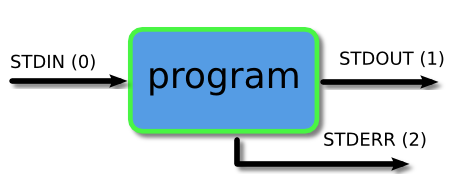
\includegraphics[width=0.5\textwidth]{redirection-std.png}
\end{figure}

\begin{minted}{bash}
# redirect the output of a command to out.txt 
# and redirect the error of the command to error.txt:
ls -la > out.txt 2> error.txt

# redirect stderr to stdout (&1), and then redirect stdout to a file out.txt:
ls -la > out.txt 2>&1

# redirect both to a file:
ls -la &> out
\end{minted}

\subsubsection{stdin}

\begin{minted}{bash}
# this command prints the amount of lines in a file
wc -l music.txt

# this command does the same
wc -l < music.txt

# this command does the same, but prints the output of wc to out.txt
wc -l < music.txt > out.txt
\end{minted}

\subsection{Jobs and process Management}

When you execute a command: a process is started

\begin{itemize}
    \item Every process gets a process ID (PID)
    \item The init process has PID 0. It starts other processes.
    \item Every process has a parent
    \begin{itemize}
        \item $\Rightarrow$ tree structure of processes
        \item Get insights into this structure with `pstree' (part of the `psmisc' package)
        \item Process stops: exit code is passed to the parent
    \end{itemize}
\end{itemize}

\begin{minted}{bash}
# report a snapshot of current processes
ps

# display a tree of processes
pstree -p
\end{minted}


\subsubsection{Exit codes}

\begin{minted}{bash}
# when a process stops:
# if bash was parent => exit code is passed to bash
# exit code is available in the $? variable:
# read contents of a variable with echo:
echo $?
0

# 0 = ended successfully without errors

# 1 = not ended successfully, there were errors
\end{minted}

\begin{minted}{bash}
# test = verify if you have rights on a file (with -r = read rights)
~$ test -r music.txt

~$ echo $?
0

~$ test -r doesnotexist

# the file doesn't exist, so it exited with code 1:
~$ echo $?
1
\end{minted}

\subsubsection{Combining commands}

= not the same as piping!

\begin{minted}{bash}
# note the difference between one and two ampersands:
# & = execute command 1, then execute command 2
# && = execute command 1, and only execute command 2 
#   if command 1 was successful (exit code = 0)

# one ampersand
test -r test.txt & echo "MCT rocks"

# two ampersands
~# test -r test.txt && echo "MCT rocks"

~# test -r doesnotexist & echo "MCT rocks"

# the first command will exit with code 1
# so the second command will not execute
~# test -r doesnotexist && echo "MCT rocks"
\end{minted}

\subsubsection{Jobs}

A job is a new process originating from the same parent

\begin{minted}{bash}
# start a command as job
tail -f /var/log/syslog &
# output appears on stdout, but process runs as a job in the background

# bring a job to the foreground
fg <index>

# stop the job, but do not terminate:
CTRL-Z
\end{minted}


\subsubsection{Inter-process Communication}

A signal is an asynchronous notification sent to a process or thread within that process
to notify that there has been an event

Signal sent to process $\Rightarrow$ OS interrupts normal execution of that process to deliver the signal

Sending a signal to a process: with the `kill' command:

\begin{minted}{bash}
# not only to kill a process, also to send other signals
kill -s <signal>
\end{minted}

\textbf{Signals}

\begin{itemize}
    \item SIGHUP - 1 - terminate (hang up)
    \item SIGINT - 2 - terminal interrupt signal
    \item SIGKILL - 9 - kill (cannot be caught or ignored)
    \item SIGTERM - 15 - termination signal
\end{itemize}

\begin{minted}{bash}
# send signal 15 to a process with the entered PID
kill -s 15 <pid>

# send signal 15 to the PID of the tail process
kill -s 15 'pidof tail'

# send signal 9 to a process with the entered PID
kill -s 9 <pid>

# kill the process with name 'tail'
pkill tail
\end{minted}


\subsection{Intermezzo: System Load}

= a number which represents the load on a computer system

\begin{itemize}
    \item Completely idle system: system load 0
    \item Each process which uses a resource or is waiting for a resource: system load + 1
    \item Gives an indication of how heavy a computer system is loaded
    \item System load is a snapshot, doesn't say anything
    \begin{itemize}
        \item System load of 17: is that a problem? No.
        \item More interesting: the evolution of the systemload over time
    \end{itemize} 
\end{itemize}

\begin{minted}{bash}
# show the system load of the last minute, last 5 minutes and last 15 minutes:
uptime

# show who is logged on and what they are doing
w

# display linux processes
top
# or better:
htop
\end{minted}

\subsection{Some useful tips}

\subsubsection{With which unique IP-addresses are there open sockets and how many?}

\begin{minted}{bash}
netstat -anpt | awk '{print $5}' | sort | uniq -c
\end{minted}

\subsubsection{TTY}

= Tele TYpewriter
= a terminal which is connected with stdin

\begin{minted}{bash}
# print the filename of the terminal currently connected to standard input:
~$ tty
\end{minted}

\subsection{Answer these questions to test your knowledge}

\begin{enumerate}
    \item What does piping mean?
    \item What is the prerequisite for using the command 'uniq'
    \item What is the difference between $>$ and $>>$
    \item Which are the 2 output streams in linux, and what do they contain?
    \item What is 'exit code'
    \item Why is the exit code useful
    \item What different values can the exit code be?
    \item What is the exit code for success?
    \item How do you request the exit code?
    \item How do you turn a command into a job?
    \item How do you pause a job
    \item What command shows the list of all running or paused jobs?
    \item How do you re-activate a paused job?
    \item What does the command screen do?
    \item What is meant by the term `signal'?
    \item How do you send a signal to a process
    \item How do you specify which process?
    \item Give 2 examples of signals
    \item Is a systemload of 23 problematic
    \item What process has PID 1?
    \item Where do you know this process from?
\end{enumerate}


\section{Regex, users \& firewall}

\subsection{Regex}

\begin{itemize}
    \item Make the webscaper assignment
    \item Use \url{www.regexr.com} to test regex
\end{itemize}

\subsection{User management}

\subsubsection{Add a user}

\begin{itemize}
    \item Root privilege required!
    \item There are two common commands to add users:
\end{itemize}

\begin{minted}{bash}
adduser testuser1
# enter password
# name, other details
# /home/testures1
# contents of this directory follows /etc/skel
# group: testuser1
# default shell = /bin/bash

useradd testuser2
# user is created , no password, no shell
\end{minted}

\subsubsection{Delete a user}

Again with root privileges, and 2 possible commands:

\begin{minted}{bash}
deluser testuser1
# user and corresponding group get deleted
# home directory not deleted

userdel testuser2
# user and corresponding group get deleted
# home directory also deleted
\end{minted}

\subsubsection{Change password of user}

\begin{minted}{bash}
# change your own password
passwd
# enter current password
# enter new password x2

# change password of other account (root privilege required)
passwd <username>
# current password not needed, only new password x2
\end{minted}

\subsubsection{Create a new group}

Root privilege required!

\begin{minted}{bash}
addgroup testgroup1
# GID = group ID

groupadd testgroup2
\end{minted}

\subsubsection{Assign a user to a group}

\begin{minted}{bash}
usermod -aG testgroup1 testuser1
# add to group, groupname, username

# overview of groups and group members
cat /etc/group

# of which groups is the current user a member?
~# groups
~# su – testuser1
~$ groups
\end{minted}

\subsubsection{Overview of users}

/etc/passwd

\begin{itemize}
    \item Username
    \item User ID
    \item Home directory
    \item Default shell
    \item Full name
    \item \dots
\end{itemize}

\subsubsection{Overview of groups}

/etc/group

\begin{itemize}
    \item Groupname
    \item Group ID
    \item Group members
\end{itemize}

\subsubsection{/etc/shadow}

\begin{itemize}
    \item System-wide host-specific configuration file (because it's in /etc/)
    \item Contains information about password length, expiration, password hash
    \begin{itemize}
        \item Mostly: sha512-hash
    \end{itemize}
    \item Assignment:
    \begin{itemize}
        \item write a one-liner
        \item Get all usernames from /etc/shadow and save them in /tmp/usernames
        \item Extract from /etc/shadow all usernames and hashes of passwords for the usernames where a hash of the password is known
    \end{itemize} 
\end{itemize}

\subsubsection{/etc/gshadow}

\begin{itemize}
    \item Contains an encrypted password for each group, as well as group membership and administrator information
    \item Group name: the name of the group
    \item Hashed password: 
    \begin{itemize}
        \item If the value of this field is !, no user is allowed to access the group using the newgrp command. 
        \item If the value of this field is !! : same things as !, but it also indicates that a password has never been set before
        \item If the value is null, only group members can log into the group
    \end{itemize}
    \item Group administrators: users who can add or remove group members using the gpasswd command
    \item Group members
\end{itemize}

\subsubsection{sudo}

\begin{itemize}
    \item Root privilege = superuser
    \item sudo = superuser do
    \item ~\$ sudo useradd jeff == ~\# useradd jeff
\end{itemize}

\begin{minted}{bash}
# decide who gets sudo rights:

# install the sudo package
apt install sudo
# change the rights
visudo
# view the changes
cat /etc/sudoers
\end{minted}

There is a sudo group:

\begin{itemize}
    \item Called sudo, sudoers or sometimes 'real'
    \item Members of sudo group have sudo rights
    \item Add user: ~\# usermod -aG sudo <username>
\end{itemize}

\subsubsection{Temporarily become another user}

\begin{minted}{bash}
sudo su - <username>
# this switches the user to <username> and use the environment of that user
# eg. the $PATH

# become root:
~$ sudo su -
# without username => root
\end{minted}


\subsection{SSH}

\underline{S}ecure \underline{SH}ell

\begin{itemize}
    \item In the past: telnet (23/TCP)
    \begin{itemize}
        \item Plain text
        \item Not feature-rich
    \end{itemize}
    \item Better: ssh (22/TCP)
    \begin{itemize}
        \item Encrypted with public-private key cryptography
        \item Feature-rich
        \item Connect through the network, login as a user and get access to the shell on the remote system as that user
        \item You're sitting at the console of that system, but with 'a very long cable'
    \end{itemize}
\end{itemize}

\subsubsection{SSH features}

\begin{itemize}
    \item Log in and get remote shell. Which shell? See /etc/passwd
    \item Invoke a command on the remote system
    \item Create a secured, encrypted tunnel
    \item Transfer files: with scp (secure copy)
\end{itemize}

\subsubsection{SCP - Secure Copy}

\begin{itemize}
    \item Transfer files over an encrypted connection (22/TCP)
    \item scp <what to copy> <where to copy to>
    \item Also specify the username, the remote system and the location on that system
\end{itemize}

\subsubsection{SSH tunnels}

Tunnel a port to let traffic through a certain port

\begin{minted}{bash}
ssh -L <local-IP>:<local-port>:<remote-ip>:<remote-port> username@ssh-server

# SOCKS-proxy functionality:
ssh -D <local-port> username@ssh_server
\end{minted}

\subsection{Full-fledged environment}

\begin{figure}[H]
    \centering
    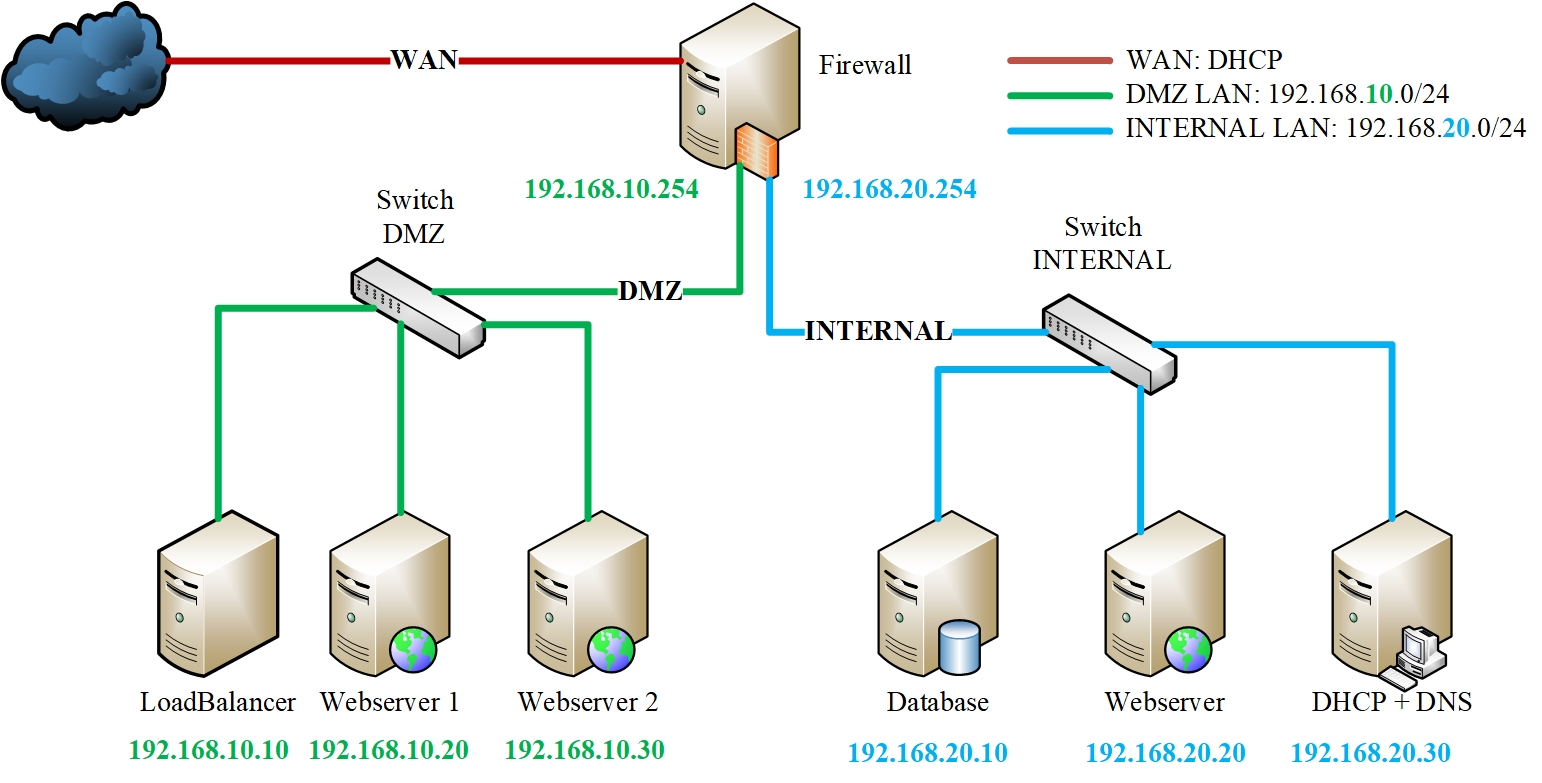
\includegraphics[width=0.7\textwidth]{full-fledged-environment.jpg}
    \caption{We will create this setup}
\end{figure}

\begin{itemize}
    \item 7 VMs
    \item Two networks: internal and DMZ network for public services
    \item A firewall
    \item NAT-ing
\end{itemize}

\subsection{Basic networking}

To create the setup in the previous section, we need to recap some basic networking:

\subsubsection{TCP/IP network model}

\begin{figure}[H]
    \centering
    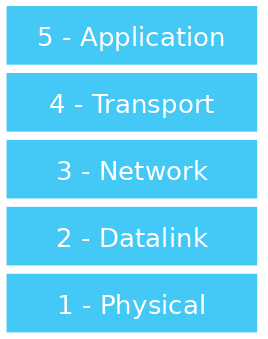
\includegraphics[width=0.25\textwidth]{tcp-ip.png}
    \caption{The 5 layers of the TCP/IP model}
\end{figure}

\begin{enumerate}
    \item Physical layer: our VMware virtual network
    \item Datalink layer: ethernet \& MAC-address
    \item Network layer: IPv4, IP-address
    \item Transport layer:
    \begin{itemize}
        \item Transport Control Protocol (TCP)
        \item User Datagram Protocol (UDP)
    \end{itemize}
    \item Application layer: SSH, HTTP, \dots
\end{enumerate}

\begin{figure}[H]
    \centering
    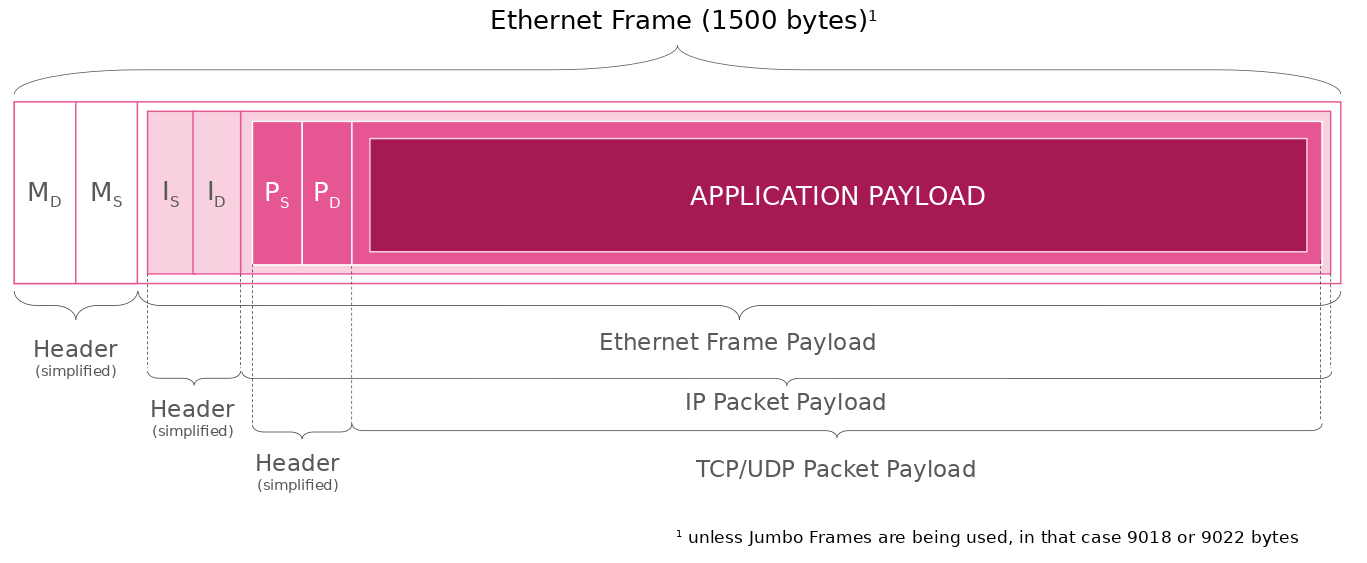
\includegraphics[width=0.84\textwidth]{tcp-ip2.png}
    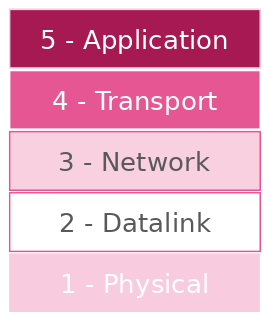
\includegraphics[width=0.15\textwidth]{tcp-ip3.png}
    \caption{An ethernet frame}
\end{figure}

\subsubsection{3 types of firewalls}

\begin{enumerate}
    \item Application Layer Gateway
    \begin{itemize}
        \item Can see layer 7
        \item Can see the application payload
    \end{itemize}
    \item Stateful Packet Inspection Firewall
    \begin{itemize}
        \item Stateful = it can keep status, it has memory
        \item Can't see the application payload
    \end{itemize}
    \item Packet Filtering Firewall
    \begin{itemize}
        \item Simplest type of firewall
        \item Can only see information up to Layer 4 (Transport layer)
        \begin{itemize}
            \item Source \& Destination MAC-address
            \item Source \& Destination IP-address
            \item Source \& Destination Port number
            \item The interface where the packet travels through
        \end{itemize}
        \item Can't see the application payload
    \end{itemize}
\end{enumerate}

\section{Netfilter, iptables}

\subsection{Intermezzo: kernel space vs user space}

System memory can be divided in 2 parts: kernel space and user space

\subsubsection{Kernel space}

\begin{itemize}
    \item Kernel space is that part of memory in which kernel processes are running
    \item Kernel space memory can not be swapped or deallocated: it is fixed
\end{itemize}

\subsubsection{User space}

\begin{itemize}
    \item AKA userland
    \item That part of the memory where user mode applications are running
    \item Can be swapped out when needed
\end{itemize}

\subsection{Intermezzo: Routing}

\begin{itemize}
    \item Firewall without ruleset = router
    \item Router with filtering = firewall
\end{itemize}

Routing = layer 3 (network)

\begin{figure}[H]
    \centering
    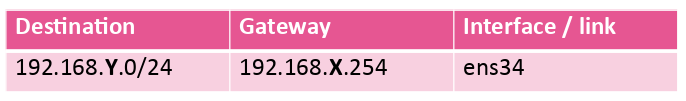
\includegraphics[width=0.4\textwidth]{routing-table.png}
    \caption{What a route looks like (netstat -rn)}
\end{figure}

Routing = road signs of the network

\begin{itemize}
    \item Town name = network
    \item Road sign = route
    \item Street = interface/link
\end{itemize}

Router = connected with multiple networks

\begin{itemize}
    \item Possibly other routers and network further down
    \item Routing table determines the path to follow
    \item Create firewall:
    \begin{itemize}
        \item First create routes
        \item Then add rules
    \end{itemize}
\end{itemize}


\subsection{Firewalls}

\subsubsection{3 types firewall}

\begin{itemize}
    \item Application Layer Gateway
    \item Stateful Packet Inspection
    \item Packet filtering
\end{itemize}

\subsubsection{Stateful Packet Inspection Firewall (SPI)}

= Packet filter + inspection of state of connection

\begin{itemize}
    \item Invented / introduced by Check Point in 1994 in FireWall-1
    \item Packet filter: \textit{stateless}
    \item Every packet evaluated individually against ruleset
    \item A lot of packets belong together => make it stateful
    \item Extra advantage: drop packets which do not belong in the flow
\end{itemize}

\begin{figure}[H]
    \centering
    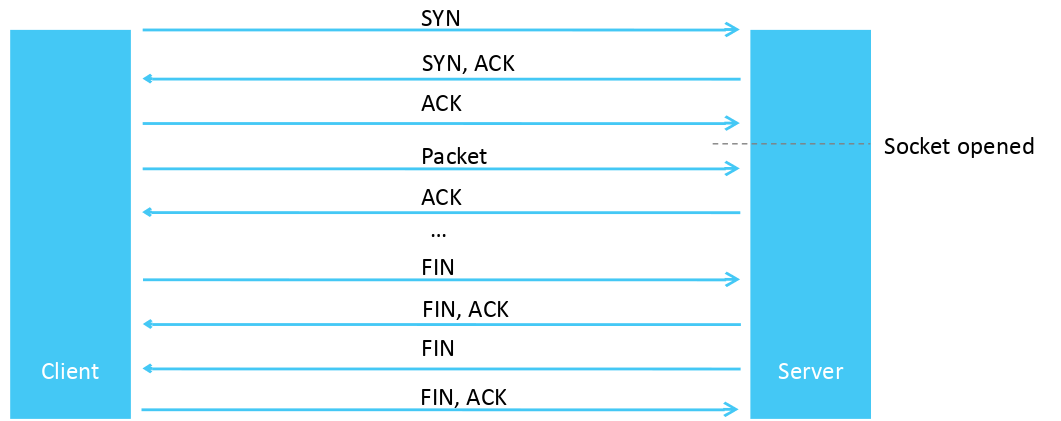
\includegraphics[width=0.5\textwidth]{stateful-packet-inspection.png}
    \caption{}
\end{figure}

\begin{itemize}
    \item 3 way handshake between client and server
    \item Socket opens
    \item Packets + ACKs
    \item \dots
    \item 4 way close
\end{itemize}

\begin{figure}[H]
    \centering
    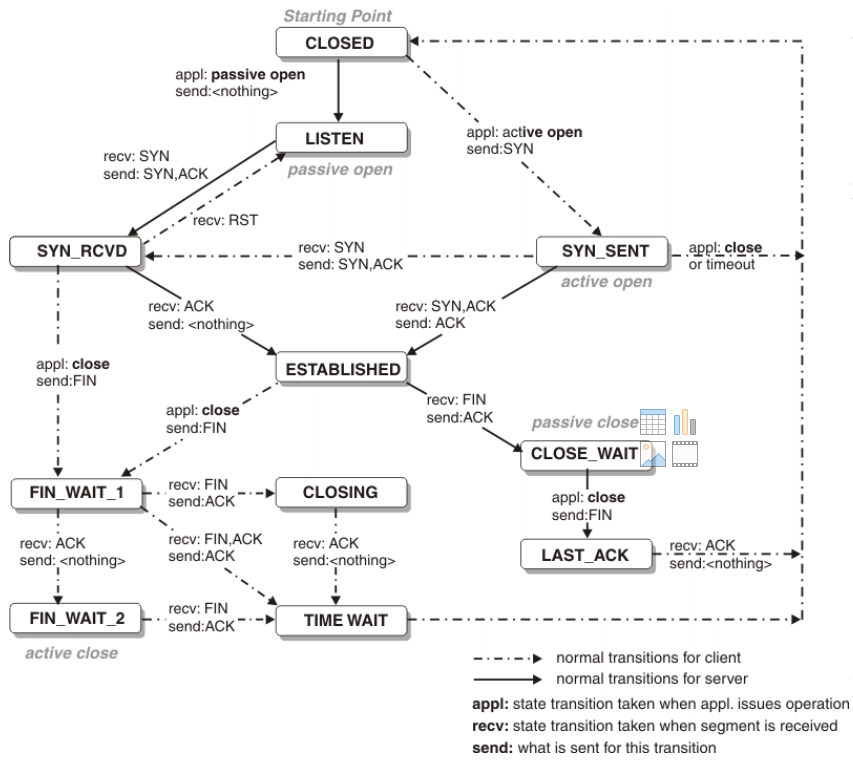
\includegraphics[width=0.5\textwidth]{flowchart-states.png}
    \caption{Flowchart of the states}
\end{figure}


Type of packet does not fit in one of the currently existing flows? $\Rightarrow$ DROP!

\begin{figure}[H]
    \centering
    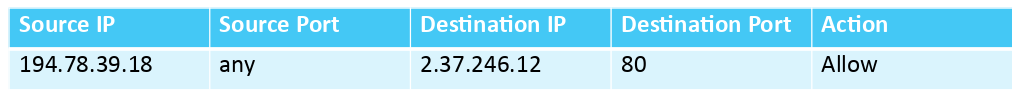
\includegraphics[width=0.5\textwidth]{spi-table.png}
    \caption{Firewall rule}
\end{figure}

Packet arrives with

\begin{itemize}
    \item sIP = 194.78.39.18
    \item sPrt = 20233
    \item dIP = 2.37.246.12
    \item dPrt = 80
    \item Flags = P (push)
\end{itemize}


$\Rightarrow$ Packet Filter firewall $\Rightarrow$ ACCEPT

$\Rightarrow$ SPI and no SYN, SYN/ACK, ACK seen before? $\Rightarrow$ DROP


\subsubsection{Stateful Packet Inspection vs Packet Filter}

Pro:

\begin{itemize}
    \item More secure
    \item Evaluate less individual packets (less CPU usage)
\end{itemize}

Cons:

\begin{itemize}
    \item Requires more memory (table with state of connections)
    \begin{itemize}
        \item Decades ago this was a problem because firewalls would only have several MBs of RAM
        \item Not a problem anymore because of servers with a lot of RAM
    \end{itemize}
\end{itemize}

\subsubsection{SPI in Linux: Connection tracking (conntrack)}

The connection tracking system stores information 
about the state of a connection in a memory structure that 
contains the source and destination IP addresses, port number pairs, 
protocol types, state, and timeout.

\begin{itemize}
    \item conntrack: part of the kernel (it's a kernel module)
    \item conntrack-tools: user space tools to interact with the in-kernel connection tracking system
    \item SPI uses the conntrack kernel module, these days it is loaded by default
\end{itemize}

\subsubsection{Application Layer Gateway (ALG)}

\begin{itemize}
    \item Can filter based on contents in Layer 5: the Application layer
    \item Has knowledge of application protocols
    \item Example:
    \begin{itemize}
        \item Active FTP
        \begin{itemize}
            \item Active FTP uses a Control Connection (21/TCP) and a Data Connection (20/TCP), for example:
            \item Client: 53621 $\Rightarrow$ Server: 21 (Control Connection: list, get, \dots)
            \item Server: 20 $\Rightarrow$ Client: 53622 (Data Connection: actual transfer)
        \end{itemize}
        \item Passive FTP
        \item HTTP: what website may be visited and what websites may not?
    \end{itemize}
\end{itemize}

Problem: more and more traffic gets encrypted:

\begin{itemize}
    \item HTTPS, SMTP + SSL, SSH, \dots
    \item One cannot `look' inside encrypted traffic
    \item Solution: SSL-inspection
    \item Purpose: SSL (client $\Rightarrow$ server)
    \item Problem:
    \begin{itemize}
        \item SSL1: client makes SSL connection to Firewall
        \item SSL2: Firewall makes second SSL connection to server
        \item The certificates for the two SSL connections are different
        \item Man In The Middle attacks on the Firewall device are possible without the client or server knowing
        \item Solution: end-to-end (E2E) encryption
    \end{itemize}
\end{itemize}

\subsubsection{Purpose of a firewall}

\begin{itemize}
    \item Selectively allow network traffic
    \item Network traffic which is welcome, may enter or may pass
    \item Traffic that is not welcome, is banned
    \item Firewall uses rules, traffic is evaluated against those rules
\end{itemize}

\subsection{Firewall in Linux: iptables}

\begin{itemize}
    \item iptables = package with userspace tools
    \item Interacts with netfilter (package filtering framework) in kernel space 
\end{itemize}

\subsubsection{Netfilter}

Networking stack = in kernel space

\begin{itemize}
    \item Driver of network interface card (NIC)
    \item Ethernet
    \item CSMA/CD
    \item Flow-Control
    \item IEEE802.11 (VLAN)
    \item \dots
\end{itemize}

These processes in kernel space are provided with a couple API hooks

\subsubsection{Hooks}

\begin{theorem}
    A hook is a functionality provided by software for users of that software
    to have their own code called under certain circumstances.

    Specific actions can be `hung' on these `hooks'

    \url{https://en.wikipedia.org/wiki/Hooking}
\end{theorem}

Specifically for netfilter hooks:

\begin{itemize}
    \item Code in the Linux kernel which can catch a specific event of a packet in the network stack
\end{itemize}

\begin{figure}[H]
    \centering
    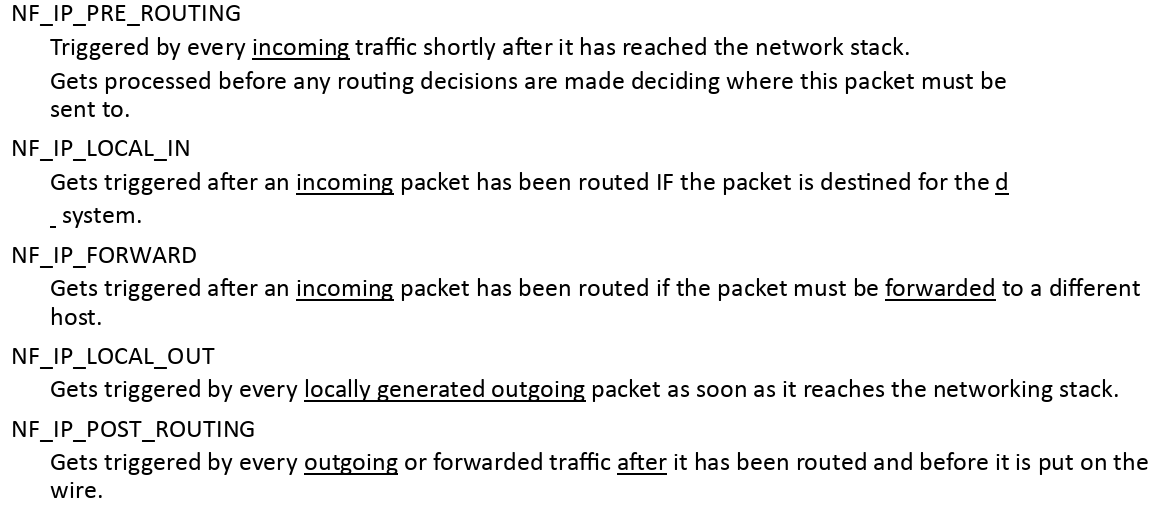
\includegraphics[width=0.5\textwidth]{hooks.png}
    \caption{5 hooks in the kernel networking stack}
\end{figure}

Example: NF\_IP\_LOCAL\_IN:

\begin{itemize}
    \item Using iptables a `rule' can be created specifying which packets may be delivered to a service in this OS, and which can't.
    \item iptables uses these netfilter hooks in the kernel
    \item Packet via hook from kernelspace (networking stack, netfilter hook) to userspace (iptables)
    \item iptables decides what has to happen to the packet and passes decision via the hook back to the kernel
\end{itemize}

\subsubsection{iptables - tables}

iptables uses tables to order firewall rules

5 built-in tables:

\begin{itemize}
    \item \textbf{Filter table}
    \begin{itemize}
        \item Most commonly used
        \item To decide if a packet is allowed to its desired destination or not
    \end{itemize}
    \item \textbf{NAT table}
    \begin{itemize}
        \item To do Network Address Translation
        \item Source NAT and/or destination NAT
    \end{itemize}
    \item Mangle table
    \begin{itemize}
        \item To alter the headers of IP-packets in transit
        \item Adjust TTL, TOS, put a label/mark, \dots
    \end{itemize}
    \item Raw table
    \begin{itemize}
        \item If you do not want Stateful Packet Inspection
        \item Directly evaluate packages instead of using states, do everything manually
    \end{itemize}
    \item Security table
    \begin{itemize}
        \item To put SELinux security context marks on packets
    \end{itemize}
\end{itemize}

\subsubsection{iptables - chains}

Within each table rules are arranged in chains

\begin{itemize}
    \item These chains represent the netfilter hooks
    \item Chains determine \textbf{when} a rule will be evaluated
    \item 5 chains in iptables:
    \begin{enumerate}
        \item PREROUTING: triggered by the NF\_IP\_PRE\_ROUTING hook
        \item INPUT: triggered by the NF\_IP\_LOCAL\_IN hook
        \item FORWARD: triggered by the NF\_IP\_FORWARD hook
        \item OUTPUT: triggered by the NF\_IP\_LOCAL\_OUT hook
        \item POSTROUTING: triggered by the NF\_IP\_POST\_ROUTING hook
    \end{enumerate}
    \item Chains allow to decide where in the path of `packet-delivery' a firewall has to evaluate a rule
\end{itemize}

There are 5 built-in tables and 5 available chains.
Is every chain available in every table?

\begin{itemize}
    \item No: security table is of no use in PREROUTING or POSTROUTING  
\end{itemize}

\begin{figure}[H]
    \centering
    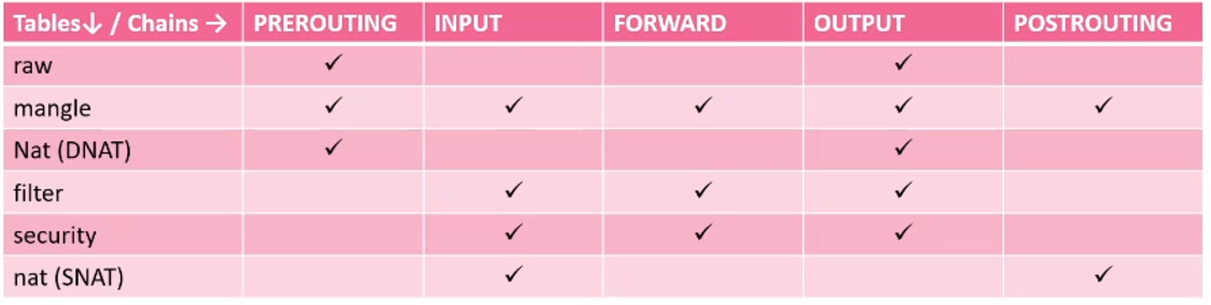
\includegraphics[width=0.5\textwidth]{iptables-tables-and-chains.png}
    \caption{Tables \& Chains}
\end{figure}

\begin{itemize}
    \item DNAT = destination NAT = Destination of IP packet gets translated
    \item Has to be done before packet gets routed $\Rightarrow$ PREROUTING
    \item The translated packet is basically a new packet which was crafted by this system and which has to leave this system $\Rightarrow$ OUTPUT
\end{itemize}

\subsubsection{Order of passing through chains}

Assumption: routing is correct and firewall allows packet

\begin{itemize}
    \item Incoming packets destined for local system: PREROUTING $\Rightarrow$ INPUT
    \item Incoming packets destined for another system: PREROUTING $\Rightarrow$ FORWARD $\Rightarrow$ POSTROUTING
    \item Outgoing locally created packets: OUTPUT $\Rightarrow$ POSTROUTING
\end{itemize}

\subsubsection{iptables rules}

Rules are places in a certain chain of a certain table

\begin{itemize}
    \item The packet gets matched with each rule from top to bottom
    \item Each rule has a `matching' component and an `action' component
    \begin{itemize}
        \item If packet matches with `this', do `that'
    \end{itemize}
\end{itemize}

\subsubsection{Targets}

The `action' component of a rule is the `target'

2 categories of targets:

\begin{itemize}
    \item Terminating targets
    \begin{itemize}
        \item Do an action that ends all further evaluation and gives control back to the netfilter hook
        \item Decision is passed on to hook: DROP or ALLOW
    \end{itemize}
    \item Non-terminating targets
    \begin{itemize}
        \item Do an action and continue with the evaluation within the chain
        \item Eventually a chain must reach a terminating target and give control back to hook
    \end{itemize}
\end{itemize}

\subsubsection{iptables and connection tracking (SPI)}

A connection can have a certain state

\begin{itemize}
    \item \textbf{NEW}
    \item \textbf{ESTABLISHED}
    \item \textbf{RELATED}
    \item INVALID
    \item UNTRACKED
    \item SNAT
    \item DNAT
\end{itemize}

\begin{figure}[H]
    \centering
    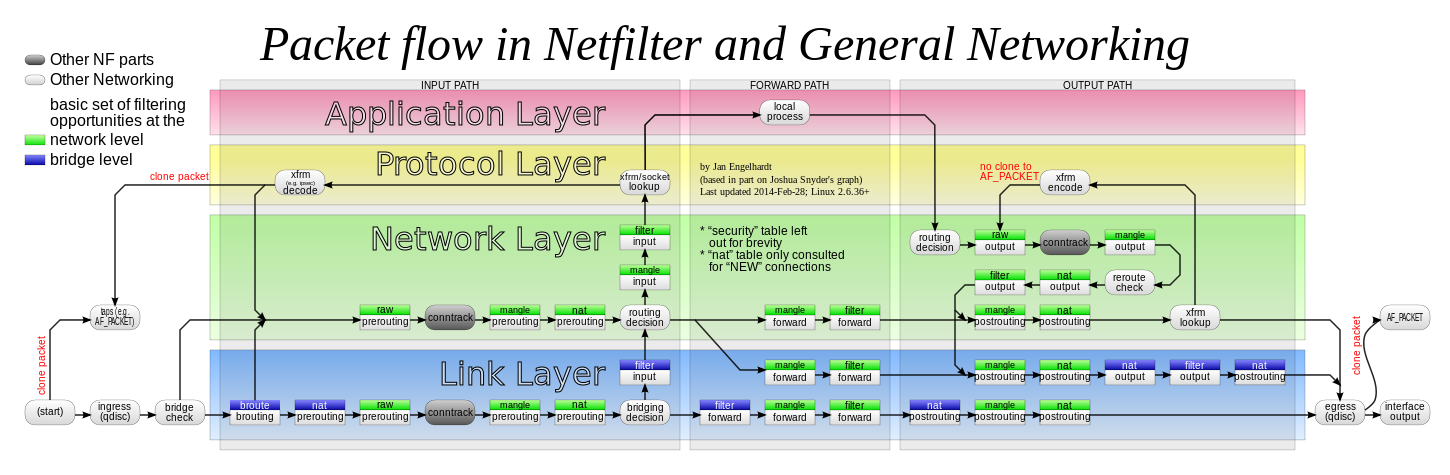
\includegraphics[width=0.5\textwidth]{packet-flow-netfilter.png}
    \caption{\url{Bron: https://en.wikipedia.org/wiki/Iptables}}
\end{figure}

\subsection{iptables in practice}

\subsubsection{Matches and Targets}

A rule is a combination of a `match' and a `target'

\textbf{Matches}

\begin{itemize}
    \item A condition that must be met for iptables to process the package
    \item Some examples:
    \begin{itemize}
        \item -s (--source): specifies the source of the packet
        \item -d (--destination): specifies the destination of the packet
        \item -p (--protocol): the protocol (e.g. tcp) which has to be matched
        \item -i (--in-interface): specifies the NIC where the packet arrives
        \item -o (--out-interface): specifies the NIC where the packet leaves
        \item ! stands for negation
    \end{itemize}
\end{itemize}

\textbf{Targets}

\begin{itemize}
    \item Determine the action which has to be taken when a packet is matched
    \item \textbf{ACCEPT:} allow the packet without further checks
    \item \textbf{DROP:} refuse the packet without sending an answer (without letting the sender know)
    \item QUEUE: pass the packet on to userspace
    \item RETURN: give the packet to the next rule in the former chain
    \item LOG: write a log entry when this rule is matched and continue
    \item \textbf{REJECT:} refuse the packet and let the sender know it was refused
\end{itemize}

\subsubsection{Inspect rule, create rules}

-A (--append): append a rule at the bottom of the ruleset
-D (--delete): remove a rule
-L (--list): show a list of all rules

\begin{minted}{bash}
~# iptables –L –nv --line-numbers

# Give a list of rules
# Don't do name resolving (-n)
# Do it verbosely (v)
# Show line numbers
\end{minted}

\subsubsection{Configure firewall: best practices}

\begin{itemize}
    \item Log in through the console
    \item Throw away all existing rules (flush)
    \item Put the default policy on DROP
    \item Allow management through the local network
    \item Start `punching holes'
\end{itemize}

\begin{minted}{bash}
# throw away all rules
~# iptables -F
\end{minted}

\begin{minted}{bash}
# Default policy DROP
# by default we don't want to allow anything
~# iptables -P INPUT DROP
~# iptables -P FORWARD DROP
~# iptables -P OUTPUT DROP
\end{minted}

\begin{minted}{bash}
# Allow management through SSH from internal LAN
# Traffic destined for this system => INPUT chain

iptables –A INPUT -s 192.168.X.0/24 
        -d 192.168.X.254 -i ens34 -p tcp -m tcp --dport 22 -j ACCEPT
\end{minted}

\section{Setting up our firewall in a full-fledged environment}

In this chapter, we will set up a firewall in this environment:

\begin{figure}[H]
    \centering
    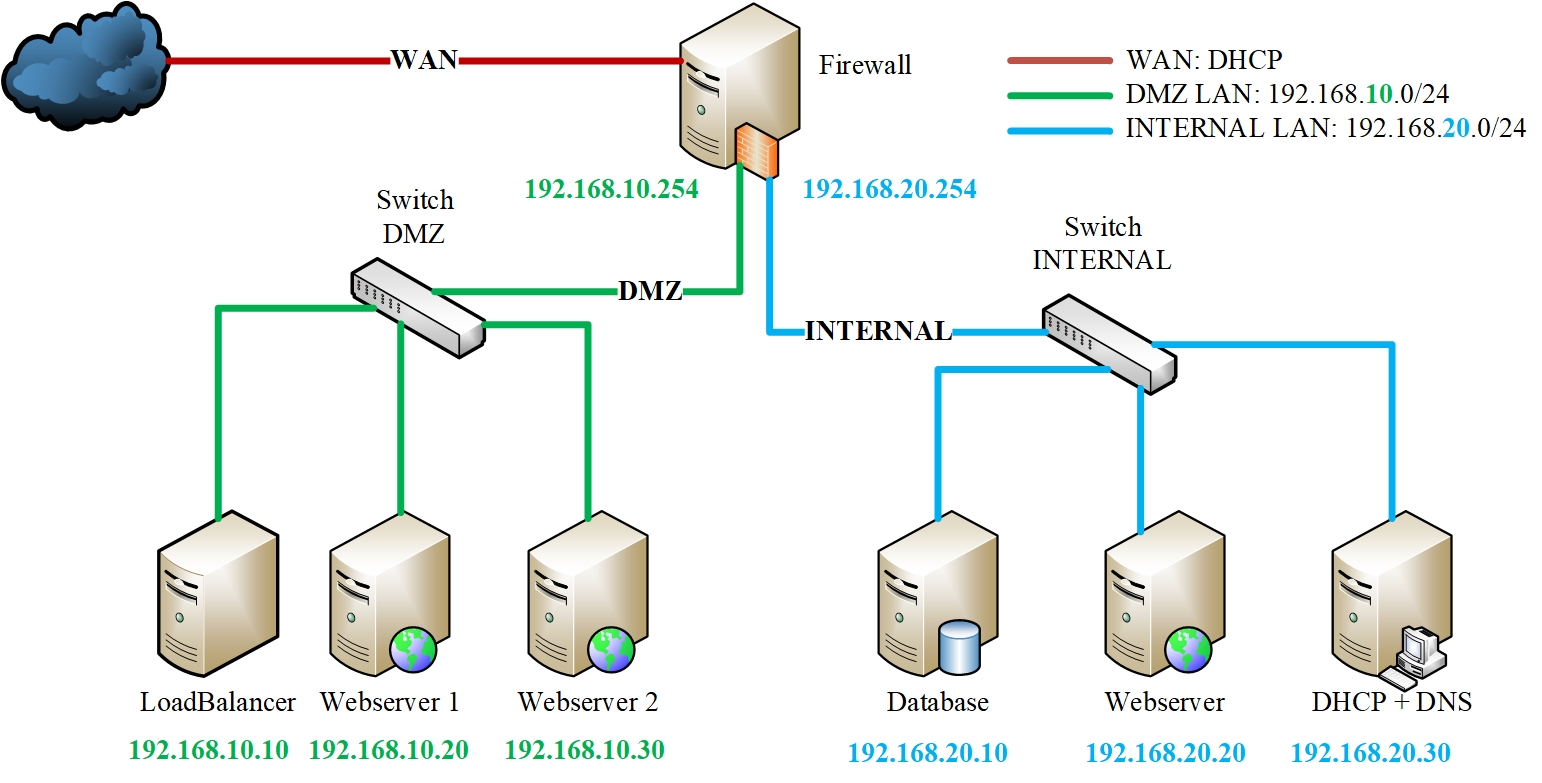
\includegraphics[width=0.7\textwidth]{full-fledged-environment.jpg}
\end{figure}

\subsection{Installation: the necessary steps}

\begin{enumerate}
    \item Forwarding: WAN / LAN / DMZ
    \begin{itemize}
        \item /proc/sys/net/ip\_forward (temporary, doesn't survive reboot)
        \item /etc/sysctl.conf (persistent)
    \end{itemize}
    \item Network interface config
    \begin{itemize}
        \item /etc/network/interfaces
        \item Configure all 3 interfaces
        \begin{figure}[H]
            \centering
            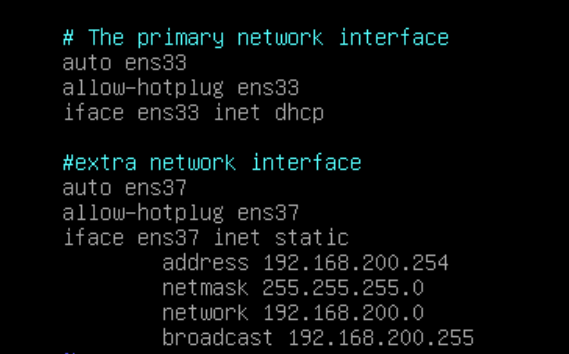
\includegraphics[width=0.4\textwidth]{etc-network-interfaces.png}
            \caption{Example}
        \end{figure}
    \end{itemize}
    \item Check interface IP configuration
    \item Check route information
    \begin{itemize}
        \item The firewall has 1 default gateway (NAT internet interface / DHCP)
        \item The 2 internal networks are directly connected
        \item Check if all are reachable with the use of \textbf{ping}
    \end{itemize}
\end{enumerate}

\subsection{iptables chains}

\begin{itemize}
    \item Standard table = filter table
    \item 3 most important chains: INPUT, OUTPUT, FORWARD
\end{itemize}


\subsubsection{INPUT chain}

= Traffic from host to firewall itself (to the processes that are running on that machine).

\begin{figure}[H]
    \centering
    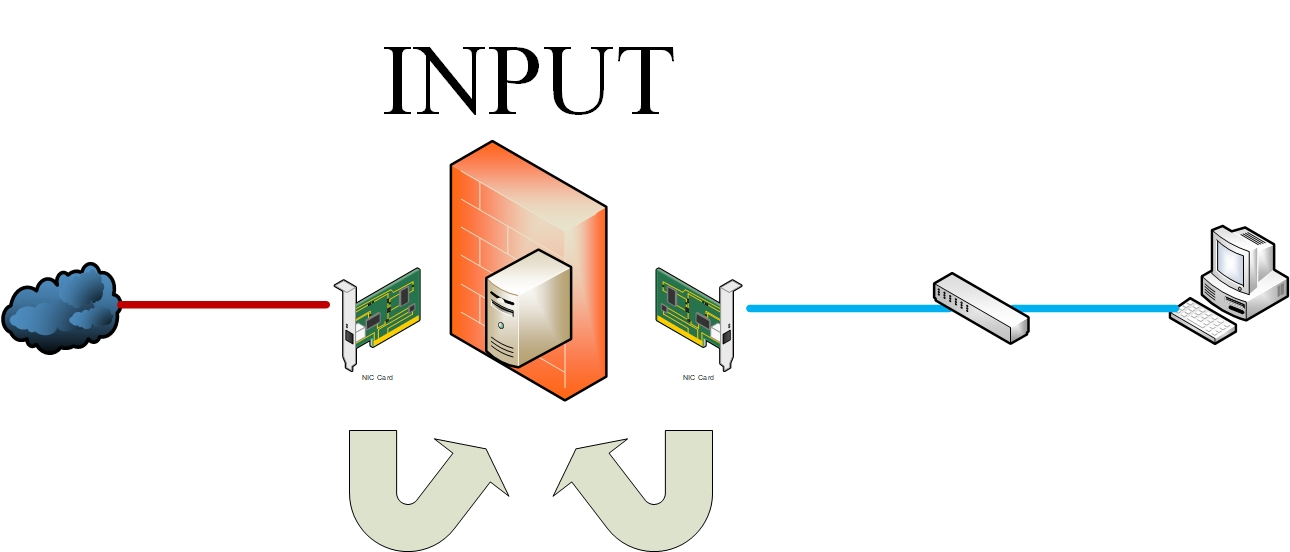
\includegraphics[width=0.5\textwidth]{input-chain.jpg}
\end{figure}

\subsubsection{OUTPUT chain}

= Traffic from firewall to host

\begin{figure}[H]
    \centering
    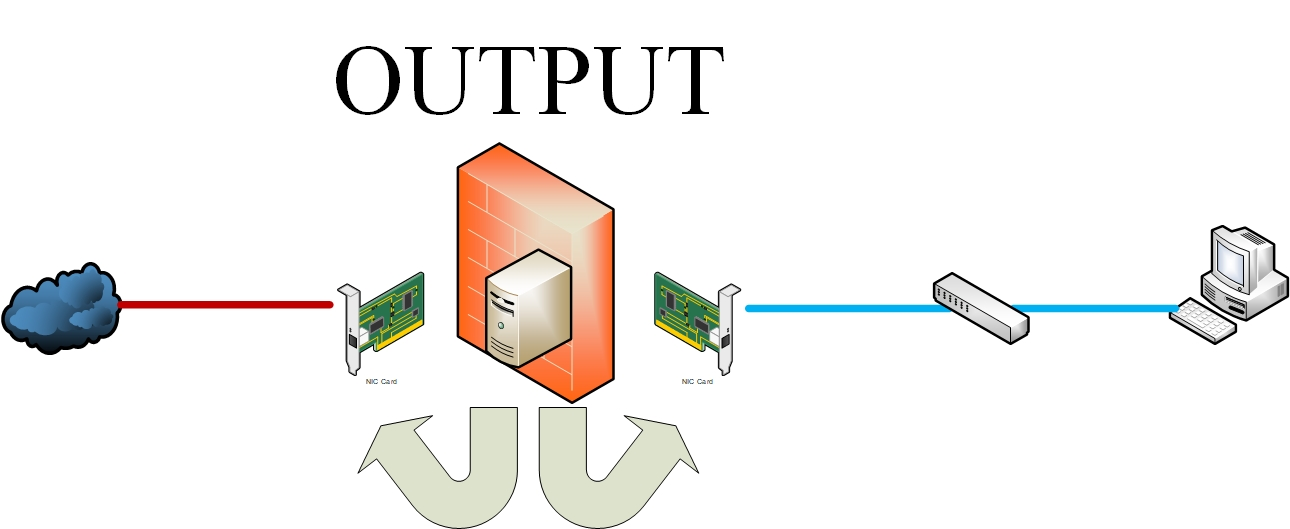
\includegraphics[width=0.5\textwidth]{output-chain.jpg}
\end{figure}

\subsubsection{FORWARD chain}

= Traffic passing through firewall from one NIC to another, or from one subnet to another.

\begin{figure}[H]
    \centering
    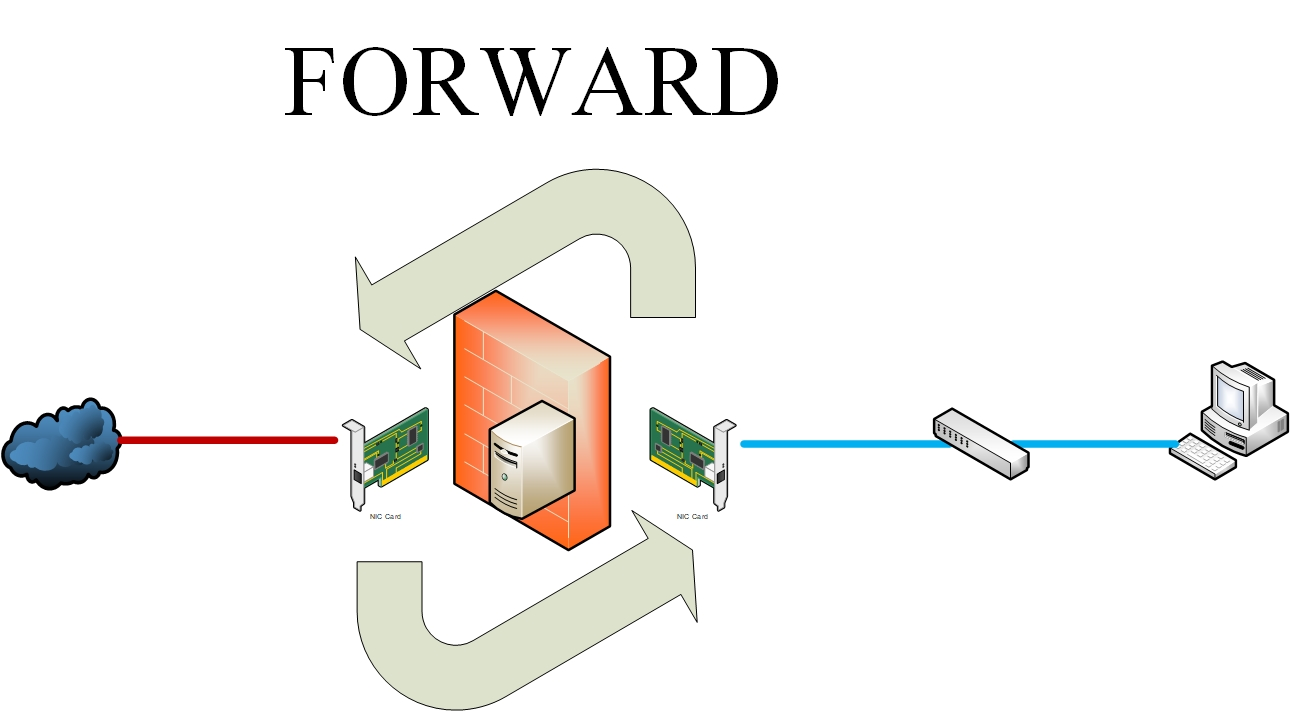
\includegraphics[width=0.5\textwidth]{forward-chain.jpg}
\end{figure}

\subsection{Common iptables commands}

\subsubsection{Clear tables}

Flush all rules:

\begin{minted}{bash}
iptables -F
\end{minted}

\subsubsection{Close firewall}

By default iptables is completely open

\begin{minted}{bash}
# close tables
iptables -P INPUT DROP
iptables -P FORWARD DROP

# keep output open
iptables -P OUTPUT ACCEPT

# why accept? 
# --> to allow traffic from firewall itself to other host
# security issue? only if firewall gets compromised
\end{minted}


\subsection{Allow SSH}

\begin{itemize}
    \item TCP traffic (port 22)
    \item Traffic from host INTO server
\end{itemize}

\begin{minted}{bash}
iptables -A INPUT -p TCP --dport 22 -s 192.168.20.0/24 -j ACCEPT
# source = 192.168.20.0/24
# accept 
# we do not specify the table, so the default is used: FILTER table
\end{minted}

\begin{itemize}
    \item Avoid connection from WAN! (to protect against brute-force attacks)
    \item IMPROVE: limit to correct incoming interface
    \begin{itemize}
        \item for example: only allow the ens33 interface
    \end{itemize}
    \item SSH = needed for daily maintenance of server
    \item What about reply?
    \begin{itemize}
        \item No problem, because OUTPUT == ACCEPT
    \end{itemize}
\end{itemize}

\subsection{Allow TCP and UDP INTO firewall}

Our current situation: our firewall blocks all incoming traffic except SSH from the 192.168.20.0/24 subnet.

\begin{itemize}
    \item Only if traffic was started FROM firewall itself
    \item $\Rightarrow$ only allow replies, never new connections
\end{itemize}

\begin{minted}{bash}
iptables -A INPUT -p TCP -m state --state RELATED,ESTABLISHED -j ACCEPT
iptables -A INPUT -p UDP -m state --state RELATED,ESTABLISHED -j ACCEPT
\end{minted}

\subsection{Allow PING or ICMP}

Why ping?

\begin{itemize}
    \item 2 way communication
    \begin{itemize}
        \item PING comes in (request)
        \item Firewall replies (reply)
    \end{itemize}
\end{itemize}

\begin{minted}{bash}
# Allow incoming ICMP connection if a host pings firewall (REQUEST)
iptables -A INPUT –p icmp --icmp-type echo-request –j ACCEPT

# Allow incoming reply if firewall pinged some host (REPLY)
iptables –A INPUT –p icmp --icmp-type echo-reply –j ACCEPT
\end{minted}

Reply or request from firewall to host:

\begin{itemize}
    \item Already OK, because OUTPUT == ACCEPT
\end{itemize}

\subsection{Internet connectivity}

\subsubsection{Who?}

\begin{itemize}
    \item For internal network \underline{through} firewall to oustide (NAT)
    \item For DMZ network \underline{through} firewall to outside (NAT)
    \item For internal network \underline{through} firewall to DMZ network (no NAT, routing)
    \item One subnet to other subnet $\Rightarrow$ one NIC to another NIC
    \item SOURCE NAT = from private local net NAT to elsewhere (public)
    \item Chain = POSTROUTING (when leaving firewall)
\end{itemize}

\subsubsection{How?}

We need to configure three things:

\begin{enumerate}
    \item Allow traffic from internal NIC to WAN NIC $\Rightarrow$ FORWARD chain
    \item Allow traffic from DMZ NIC to WAN NIC $\Rightarrow$ FORWARD chain
    \item Configure an iptable rule for NAT
\end{enumerate}

\begin{minted}{bash}
# syntax == sudo iptables -A FORWARD -i <in-interface> -o <out-interface> -j ACCEPT
# example: 
iptables -A FORWARD -i ens37 -o ens33 -j ACCEPT

# or: it always goes out on WAN NIC:
iptables -A FORWARD -o ens33 -j ACCEPT
\end{minted}

\begin{figure}[H]
    \centering
    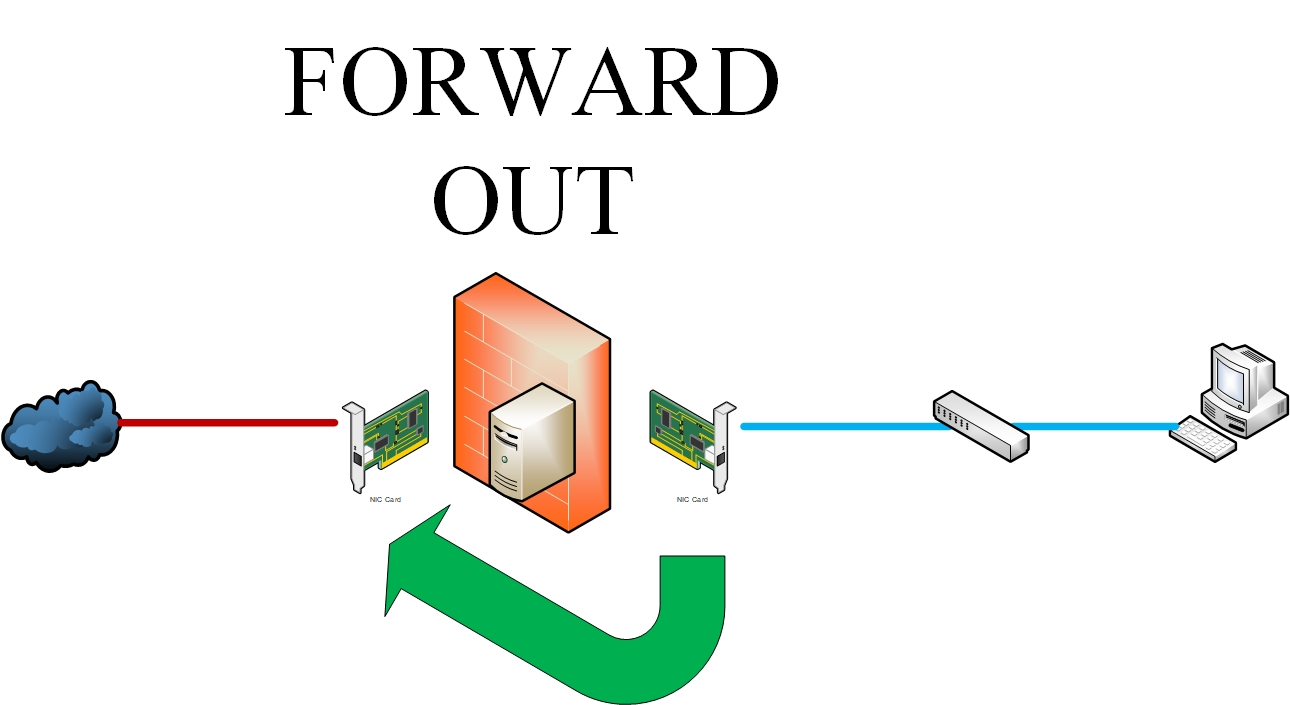
\includegraphics[width=0.5\textwidth]{forward-out-chain.jpg}
\end{figure}

\begin{itemize}
    \item iptable rule for NAT
    \item Not in FILTER table, but in our NAT table
    \item POSTROUTING chain
\end{itemize}

\begin{minted}{bash}
# syntax == sudo iptables -t nat -A <chain> -o <out-interface> -j MASQUERADE]
# example:
iptables -t nat -A POSTROUTING -o ens33 -j MASQUERADE
# -j MASQUERADE will MASQ your internal IP by using external IP
\end{minted}

\begin{figure}[H]
    \centering
    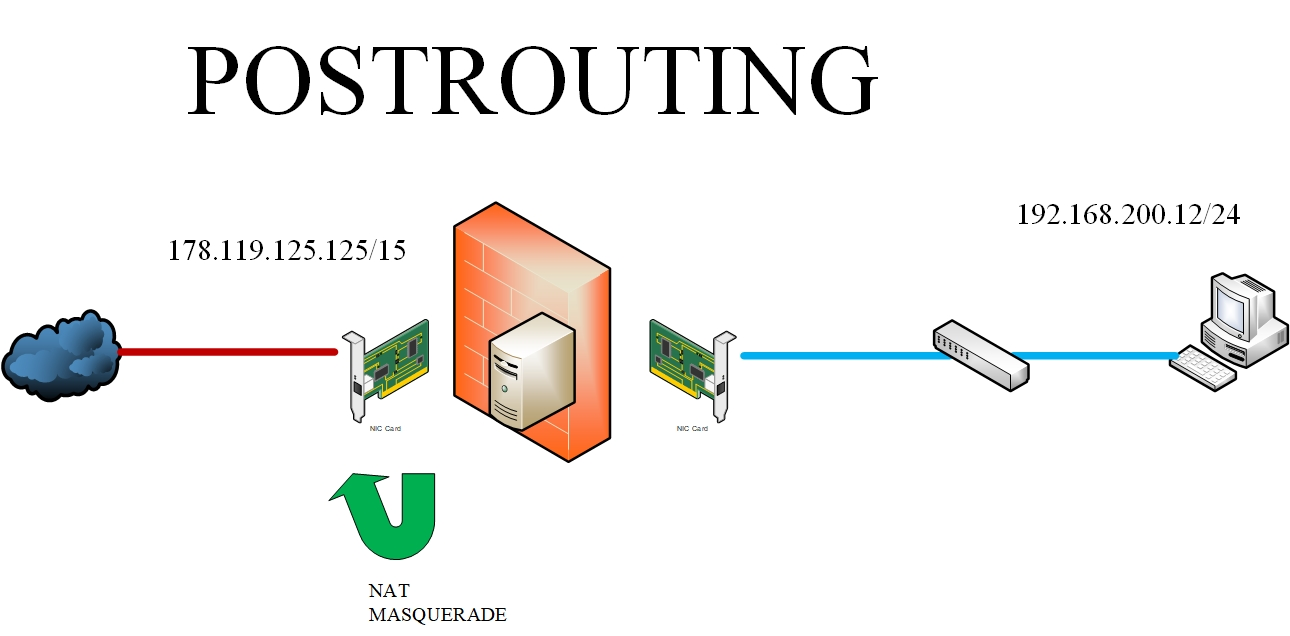
\includegraphics[width=0.5\textwidth]{postrouting-chain.jpg}
\end{figure}

\subsubsection{Allow returning traffic}

Traffic that returns and is for internal LAN or for DMZ

\begin{minted}{bash}
# allow through firewall, only if related or established traffic
iptables -A FORWARD -i ens33 -m state --state RELATED,ESTABLISHED -j ACCEPT
\end{minted}

\begin{figure}[H]
    \centering
    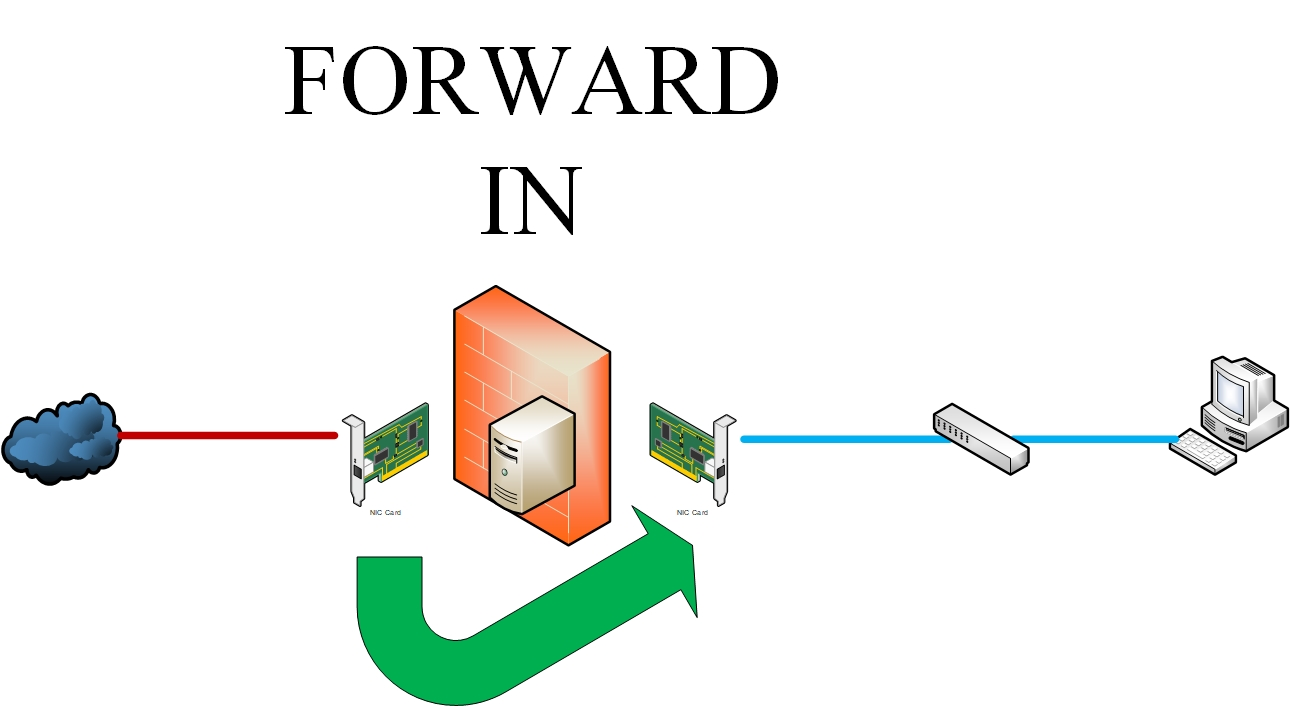
\includegraphics[width=0.5\textwidth]{forward-in-chain.jpg}
\end{figure}

\subsection{Webserver}

Traffic from internet to WAN interface, with destination a webserver in the DMZ network

\subsubsection{PREROUTING}

\begin{itemize}
    \item We need to catch WAN traffic on WAN interface ens33
    \item TCP port 80
    \item Prepare it for transport to internal network
    \begin{itemize}
        \item Change public IP to private (internal) IP
        \item = PORT FORWARDING
    \end{itemize}
\end{itemize}

\begin{minted}{bash}
# tell the PREROUTING chain: route all incoming traffic for the WAN interface, 
# TCP port 80 to an internal ip and port
iptables -t NAT -A PREROUTING -i ens33 -p tcp --dport 80 -j DNAT 
    --to-destination 192.168.10.10:80
\end{minted}

\begin{figure}[H]
    \centering
    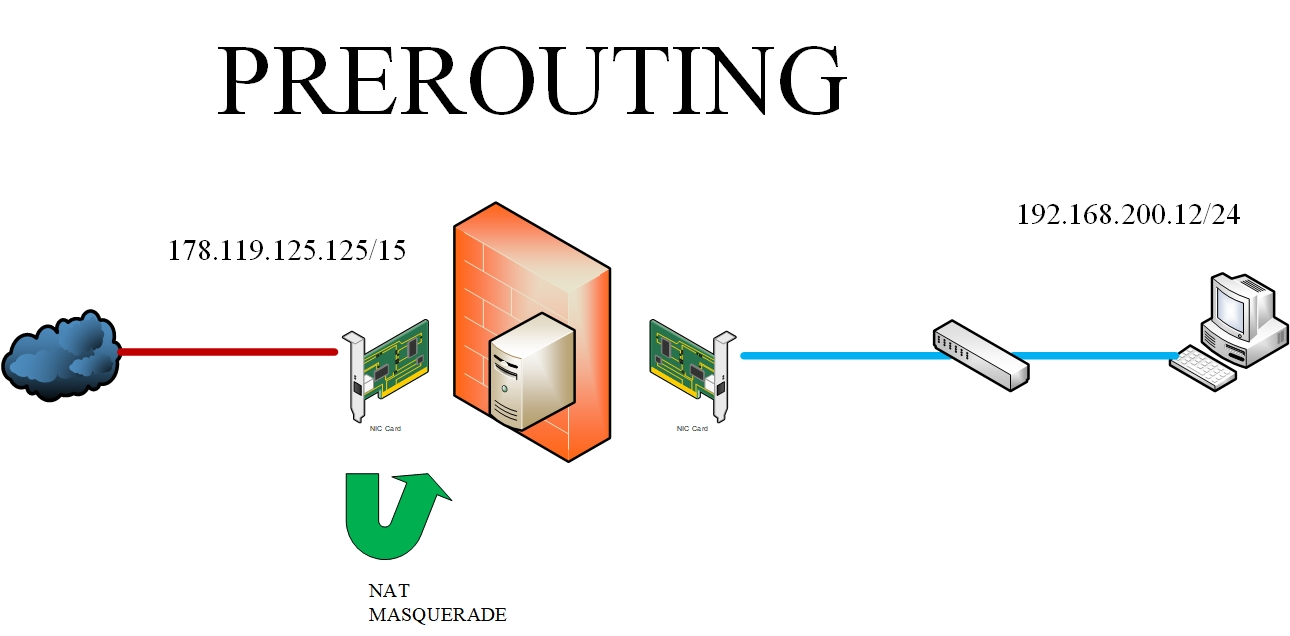
\includegraphics[width=0.5\textwidth]{prerouting-chain.jpg}
\end{figure}

\subsubsection{WAN traffic to internal webserver}

\begin{itemize}
    \item Problem: now firewall blocks this
    \begin{itemize}
        \item Is a 'new' connection, not a reply
        \item It only allows related and established connections
    \end{itemize}
    \item Solution: 
    \begin{itemize}
        \item Open TCP port 80
    \end{itemize}
\end{itemize}

\begin{figure}[H]
    \centering
    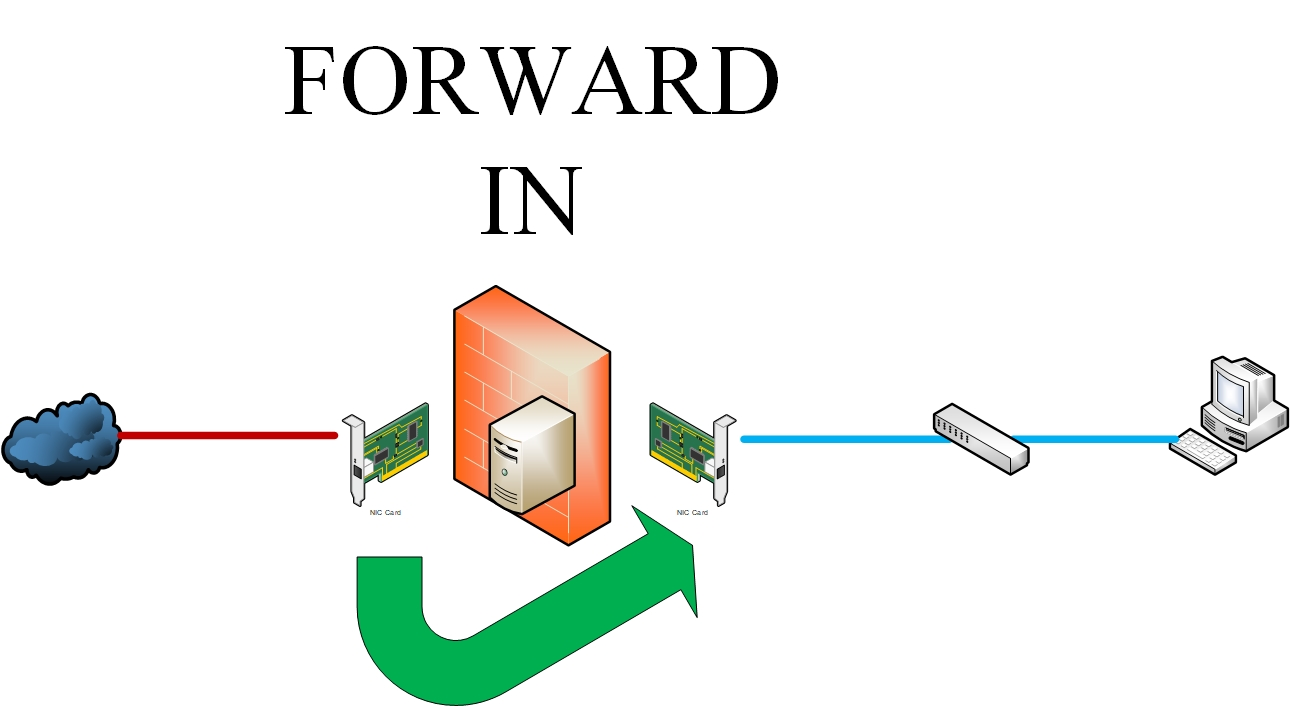
\includegraphics[width=0.5\textwidth]{forward-in-chain.jpg}
\end{figure}


\subsection{\textcolor{red}{Don't forget to save!}}

\begin{itemize}
    \item All iptables changes are in memory
    \item Changes disappear on next reboot
\end{itemize}

\begin{minted}{bash}
# command to save the iptables changes
# !! needs the iptables-persistent and netfilter-persistent packages !!
sudo netfilter-persistent save
\end{minted}

\section{DHCP}

\begin{itemize}
    \item Works with UDP
    \item Ports 67 and 68
    \item Broadcast: because the client does not have an IP address yet
    \item DHCP servers are limited to their own subnet (layer 2)
\end{itemize}

\begin{figure}[H]
    \centering
    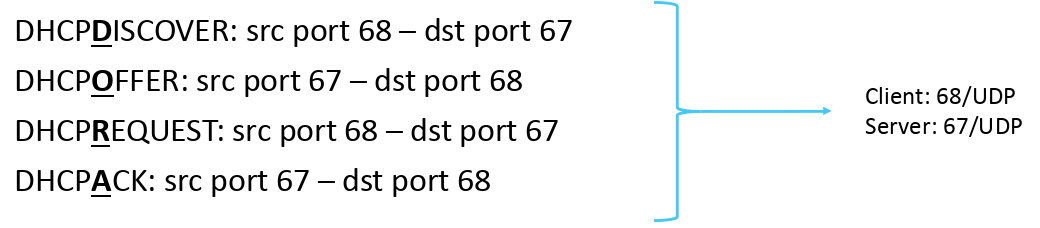
\includegraphics[width=0.5\textwidth]{dhcp-dora.png}
    \caption{Server = 67, Client = 68}
\end{figure}

\subsection{Installing a DHCP server}

\begin{itemize}
    \item Package = isc-dhcp-server
    \item ISC = Internet Systems Consortium 
    \item \url{https://www.isc.org/mission/}
\end{itemize}

\begin{minted}{bash}
~$ sudo apt install isc-dhcp-server
\end{minted}

\subsubsection{Configuration file}

\begin{itemize}
    \item System-wide host-specific configuration file $\Rightarrow$ somewhere under /etc/
    \item /etc/default/isc-dhcp-server
    \item In this file you need to allow dhcp to run
\end{itemize}

\subsubsection{Parameters to configure}

\begin{itemize}
    \item Listen on which NIC?
    \item domain-name
    \item domain-name-servers
    \item subnet
    \begin{itemize}
        \item Network address and netmask
        \item dhcp-range
        \item default gateway
    \end{itemize}
\end{itemize}

\subsubsection{Example configuration}

/etc/default/isc-dhcp-server:

\begin{minted}{bash}
INTERFACESv4="ens34"
\end{minted}

/etc/dhcp/dhcpd.conf:

\begin{minted}{bash}
subnet 192.168.20.0 netmask 255.255.255.0 {
    range 192.168.20.50  192.168.20.100;
    option routers 192.168.20.254;
    option domain-name "mctinternal.be";
    option domain-name-servers 192.168.20.30;
}
\end{minted}

\subsubsection{Dynamic vs static assignments}

Dynamic:

\begin{itemize}
    \item Available IP from the range gets assigned
\end{itemize}

Static:

\begin{itemize}
    \item Host with MAC-address X:Y:Z always has to receive IP address a.b.c.d
    \item Note: a.b.c.d lies outside the range, but inside the subnet!
\end{itemize}

\begin{minted}{bash}
host nameOfTheHost {
    hardware ethernet c8:f7:33:22:c6:4e;
    fixed-address 192.168.20.200;
}
\end{minted}

\subsection{Intermezzo: high availability}

\begin{itemize}
    \item Purpose: increase the availability of a service
    \item How? Build in redundancy
    \item Redundancy = overcapacity
    \item In other words: create overcapacity and ensure that it does not oppose each other
\end{itemize}

\subsubsection{Active-Passive clustering}

\begin{itemize}
    \item One server is active and serves clients
    \item The other server is passive and only intervenes when the active one fails
    \item The passive server periodically syncs with the changes from the active server
    \item Or every transaction is synced to both servers at the same time
    \item $\Rightarrow$ `Referee' required
\end{itemize}

\subsubsection{Split-brain}

With most types of clustering, there is a possible problem. Take the following situation:

\begin{itemize}
    \item Active still works
    \item Passive still works
    \item But they don't know it from each other
    \item $\Rightarrow$ passive thinks active is gone and becomes active
    \item Problem: 2 active servers $\Rightarrow$ many problems
\end{itemize}

\subsubsection{STONITH}

\begin{itemize}
    \item A way of `fencing' with clusters
    \item = Shoot The Other Node In The Head
    \item \url{https://en.wikipedia.org/wiki/STONITH}
    \item You provide a mechanism to `kill' one node once the other node takes over
    \item Common fencing mechanisms:
    \begin{itemize}
        \item Shutting down the UPS to the server
        \item Hardware-wise shut down the network
    \end{itemize}
\end{itemize}

\subsubsection{Highly available DHCP server}

\begin{itemize}
    \item 2 DHCP servers in network $\Rightarrow$ Many possible problems:
    \begin{itemize}
        \item If they have incompatible configurations
        \item If they have the exact same configurations
    \end{itemize}
\end{itemize}

Solution: a High Availability (HA) DHCP server

\begin{itemize}
    \item With a HA DHCP server, it is possible to `share' DHCP configuration among multiple servers
    \item Let the HA DHCP server fix its own problems 
\end{itemize}

Easier solution:

\begin{itemize}
    \item 2 DHCP servers with the same configuration
    \item Except the subnet range: make sure the subnet range do not overlap
\end{itemize}

\subsection{DNS Server}

\subsubsection{Properties of DNS}

\begin{itemize}
    \item 53/UDP (normal use)
    \item 53/TCP (zone transfer, or as a fallback for UDP)
    \item Resource Records (RR)
    \item FQDN, with a trailing dot at the end
    \begin{itemize}
        \item For example: `www.example.com.'
        \item \url{http://www.dns-sd.org/TrailingDotsInDomainNames.html}
    \end{itemize}, 
    \item 2 types of DNS queries:
    \begin{itemize}
        \item Iterative queries: the DNS server will not go and fetch the complete answer for your query but will give back a referral to other DNS server’s, which might have the answer.
        \item Recursive queries: queries in which the DNS server, who received your query, will do all the job of fetching the answer and giving it back to you.
    \end{itemize}
\end{itemize}

\subsubsection{Structure of a DNS packet}

\begin{figure}[H]
    \centering
    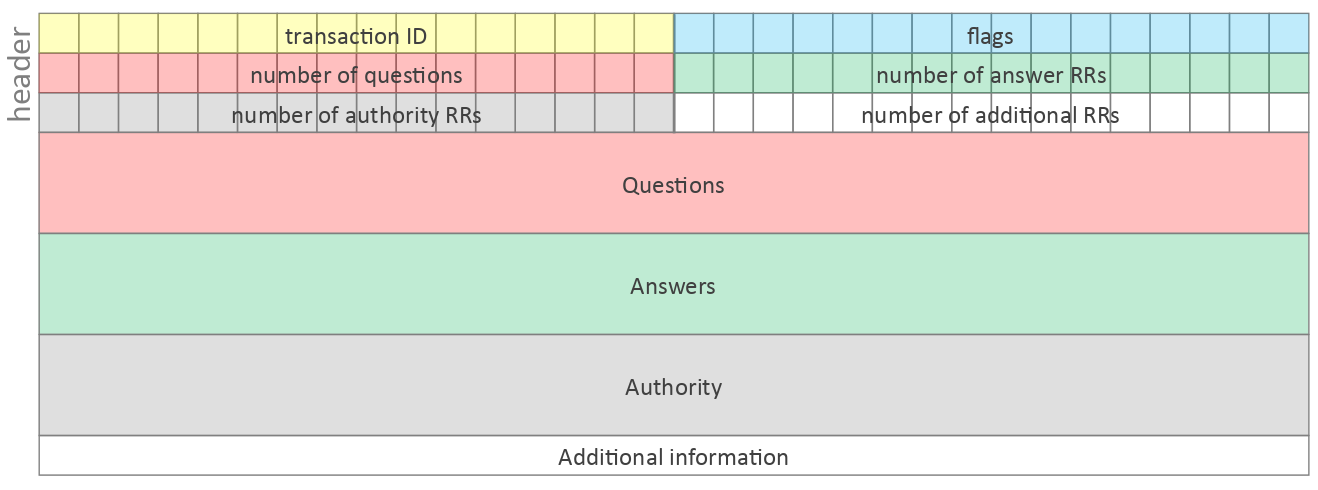
\includegraphics[width=0.5\textwidth]{dns-structure.png}
    \caption{Structure of a DNS packet}
\end{figure}

\subsubsection{DNS Records}

\begin{itemize}
    \item Convert hostnames into IP-address = \textbf{A-record}
    \item Convert IP address into hostname = \textbf{PTR-record}
    \item What server does e-mail for this domain = \textbf{MX-record}
    \item Anti-SPAM = \textbf{SPF-record} (using a specifically formatted TXT-record)
    \item What server does DNS for the domain = \textbf{NS-record}
    \item Alias of another A-record = \textbf{CNAME}
\end{itemize}

\subsection{DNS in Debian GNU/Linux}

\subsubsection{DNS Client}

\begin{itemize}
    \item Using the `dig' command, you can query DNS servers
    \item There are many parameters to filter/change the query:
    \begin{itemize}
        \item dig ns www.nmct.be $\Rightarrow$ query only NS-records
        \item +norecurse $\Rightarrow$ don't use recursive queries
        \item You can query a specific DNS server: dig @ns1.example.com www.example.com
    \end{itemize}
\end{itemize}

\begin{figure}[H]
    \centering
    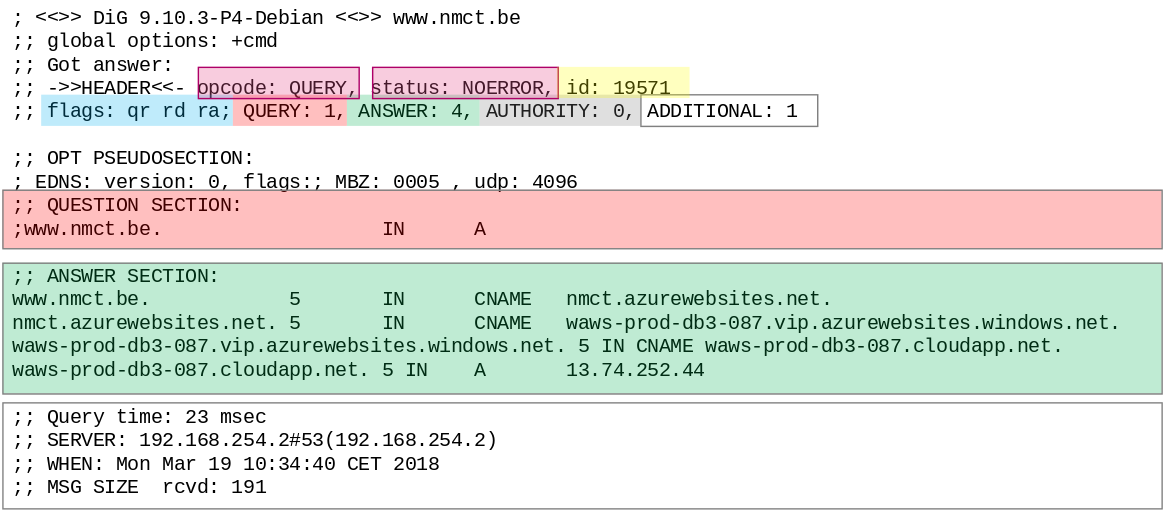
\includegraphics[width=0.5\textwidth]{dig1.png}
    \caption{dig www.nmct.be}
\end{figure}

\begin{figure}[H]
    \centering
    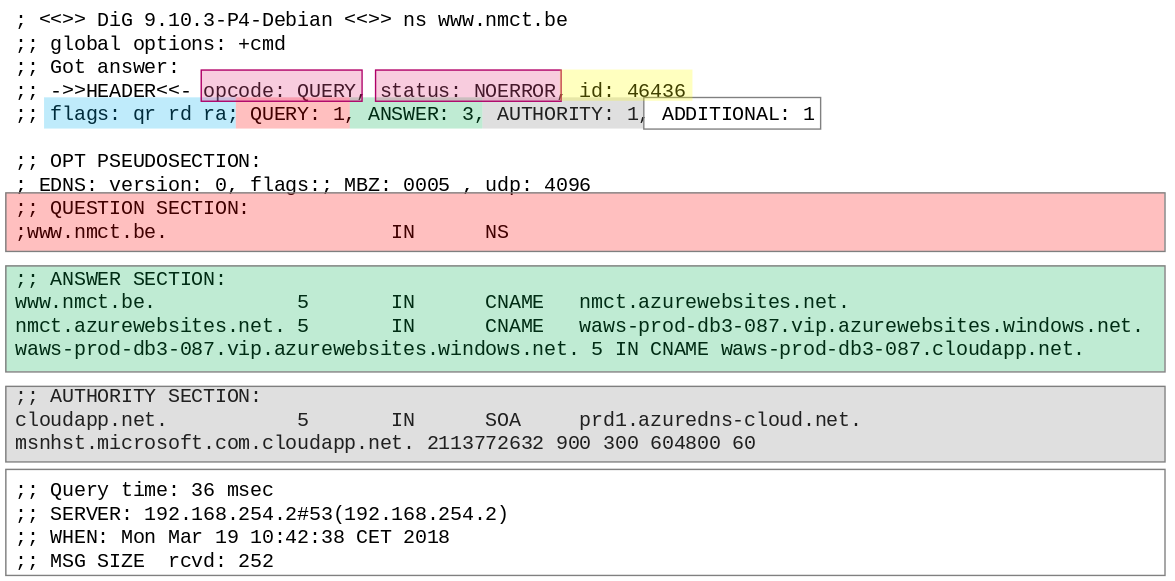
\includegraphics[width=0.5\textwidth]{dig2.png}
    \caption{dig ns www.nmct.be $\Rightarrow$ query NS-records}
\end{figure}

\begin{figure}[H]
    \centering
    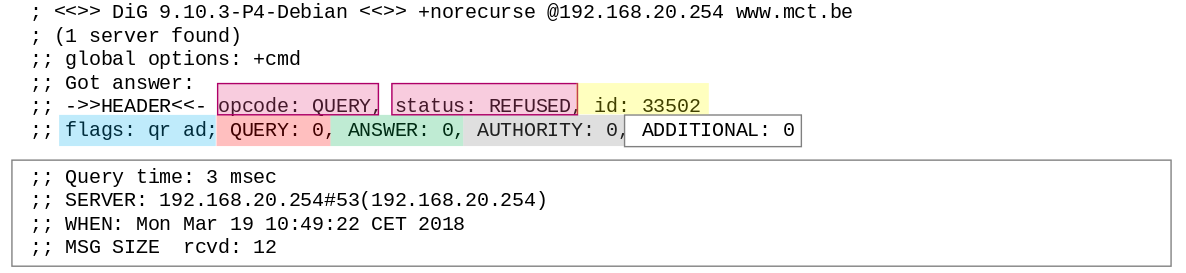
\includegraphics[width=0.5\textwidth]{dig3.png}
    \caption{dig +norecurse @192.168.20.254 www.mct.be}
\end{figure}

\begin{figure}[H]
    \centering
    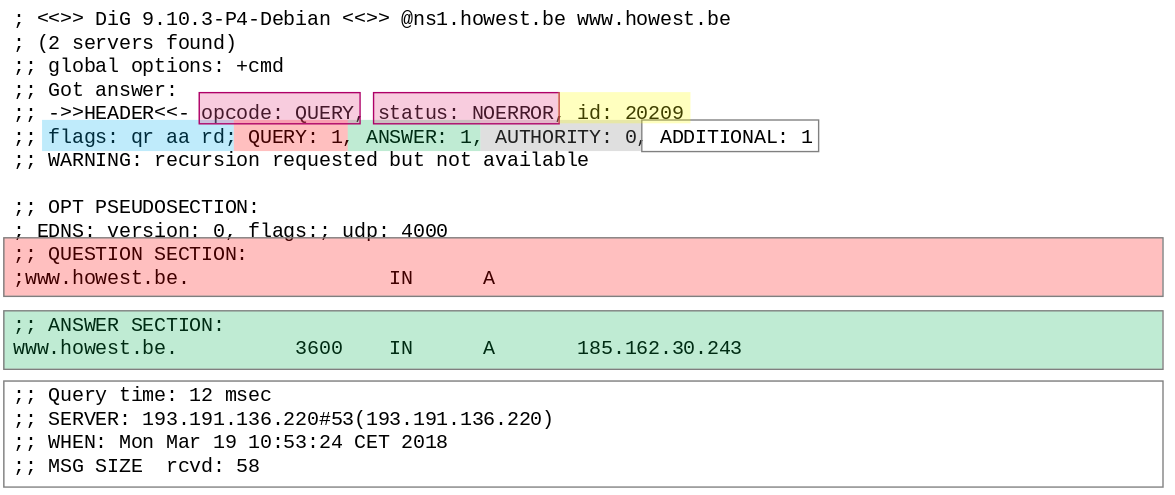
\includegraphics[width=0.5\textwidth]{dig5.png}
    \caption{dig @ns1.howest.be www.howest.be $\Rightarrow$ query a specific DNS server}
\end{figure}

\subsubsection{DNS Server}

The standard, most popular DNS server is \textbf{Bind}

\begin{minted}{bash}
# install the necessary bind packages
sudo apt install bind9 bind9utils bind9-doc

# this file holds information on root name servers
# needed to initialize cache of internet domain name servers
cat /etc/bind/db.root

# activate the bind
/etc/default/bind9
    OPTIONS="-4 -u bind"

# configuration
/etc/bind/named.conf.local 
    zone "example.com" {
        type master;
        file "/etc/bind/zones/example.com";
    };

    zone "20.168.192.in-addr.arpa" {
        type master;
        file "/etc/bind/zones/reverse/rev.20.168.192";
    };

\end{minted}

\begin{minted}{bash}
# create a zones folder, and a zones/reverse folder
sudo mkdir -p /etc/bind/zones/reverse

# contents of a zone file:
/etc/bind/zones/example.com
    ;
    ; BIND data for example.com
    ;
    $TTL 3h
    @       IN      SOA     ns1.example.com. admin.example.com. (
                            1       ; SERIAL
                            3h      ; Refresh
                            1h      ; Retry
                            1w      ; Expire
                            1h )    ; Minimum
    ;
    @       IN      NS      ns1.example.com.
    @       IN      NS      ns2.example.com.

    example.com.      IN      A       192.168.20.30
    ns1                     IN      A       192.168.20.30
    ns2                     IN      A       192.168.20.31
    www                     IN      CNAME   example.com.
    ftp                     IN      CNAME   example.com.
\end{minted}

\begin{minted}{bash}
# contents of a reverse zone file:
/etc/bind/zones/reverse/rev.20.168.192
    ;
    ; BIND reverse file for 20.168.192.in-addr.arpa
    ;
    $TTL    604800
    @       IN      SOA     ns1.example.com. admin.example.com. (
                                    1       ; Serial
                                    3h      ; Refresh
                                    1h      ; Retry
                                    1w      ; Expire
                                    1h )    ; Minimum
    ;
    @       IN      NS      ns1.example.com.
    @       IN      NS      ns2.example.com.

    38      IN      PTR     example.com.
\end{minted}


\subsection{3 useful tips}

\subsubsection{Asynchronous routing and SPI}

Be careful with asynchronous routing and Stateful Packet Inspection

\begin{itemize}
    \item SYN arrives through side A
    \item SYN, ACK leaves through side B
    \item ACK arrives through side A
\end{itemize}

\subsubsection{Make brute force on your SSH-daemon harder}

\begin{minted}{bash}
iptables -A INPUT -s 192.168.20.0/24 -d 192.168.20.201/32 
    -i eth0 -p tcp -m tcp --dport 22 -j ACCEPT

iptables -A INPUT -i eth0 -p tcp -m tcp --dport 22 
    -m state --state NEW -m recent --update --seconds 60 --hitcount 4 
    --name DEFAULT --mask 255.255.255.255 --rsource -j DROP
\end{minted}

\subsubsection{DansGuardian}

\begin{itemize}
    \item Software designed to control which websites users can access
    \item It also includes virus filtering and usage monitoring features
    \item \url{https://en.wikipedia.org/wiki/DansGuardian}
\end{itemize}

\section{Webserver \& Loadbalancer}
\subsection{Apache}

Apache is not just a webserver: Apache is a gigantic software project with:

\begin{itemize}
    \item 28 categories
    \item 185 individual projects
    \item One of which is `HTTP server' (aka httpd)
    \item \url{https://www.apache.org/index.html#projects-list}
    \item \url{http://httpd.apache.org/}
    \item Apache has its own license 
\end{itemize}

\subsubsection{History}

\begin{itemize}
    \item 1989 
    \begin{itemize}
        \item Tim Berners-Lee writes a proposal for an `information management system'
        \item Together with Belgian Robert Cailliau
        \item HyperText Transfer Protocol (HTTP)
        \item Founder of websites on the internet
    \end{itemize}
    \item Early 1990s
    \begin{itemize}
        \item World Wide Web is gradually emerging
    \end{itemize}
    \item 1995: many dissatisfied with the quality of the existing web servers
    \begin{itemize}
        \item Student projects, no real commercial webservers yet
        \item An alliance of programmers decides to create a web server themselves
    \end{itemize}
\end{itemize}

Because Apache was a gathering of work by many, there were a lot of `holes' in the code

\begin{itemize}
    \item Many `patches' had to be released to close those `holes'
    \item Hence the name = A patchy webserver
\end{itemize}

\subsubsection{Apache modules}

Apache has a modular design

\begin{itemize}
    \item Extra functionality wanted $\Rightarrow$ load module
    \begin{itemize}
        \item mod\_proxy
        \item mod\_rewrite
        \item mod\_ssl
        \item \dots
        \item \url{https://httpd.apache.org/docs/2.4/mod/}
    \end{itemize}
\end{itemize}

\begin{minted}{bash}
# get list of currently loaded modules
apache2ctl -M
\end{minted}

Which modules are enabled on your system?

\begin{minted}{bash}
/etc/apache2/mods-enabled/
# this is full of symbolic links
# don't change these links, modules are enabled/disabled with commands
a2enmod
a2dismod
\end{minted}

\subsubsection{File structure}

System-wide host-specific configuration files: /etc/apache2/

\begin{itemize}
    \item Configuration
    \begin{itemize}
        \item conf-available
        \item conf-enabled
    \end{itemize}
    \item Modules
    \begin{itemize}
        \item mods-available
        \item mods-enabled
    \end{itemize}
    \item Sites
    \begin{itemize}
        \item sites-available
        \item sites-enabled
    \end{itemize}
\end{itemize}

DocumentRoot = /var/www/html

\subsubsection{Multiple websites on 1 server: possible?}

\begin{itemize}
    \item Using VirtualHosts
    \item Every VirtualHost has a DocumentRoot
    \begin{itemize}
        \item = The folder containing the website's files
    \end{itemize}
\end{itemize}

\subsubsection{Basic Authentication}

Using 2 files:

\begin{itemize}
    \item .htaccess
    \item .htpasswd
\end{itemize}


\subsection{Intermezzo: Loadbalancing algorithms}

3 important load-balancing algorithms:

\begin{itemize}
    \item Round-robin
    \item Least connections
    \item Source
\end{itemize}

\subsubsection{Round-robin (RR)}

= Alternate between each backend server

Example with 3 servers:

\begin{itemize}
    \item 1st request goes to server 1
    \item 2nd request goes to server 2
    \item 3rd request goes to server 3
    \item 4th request goes to server 1
    \item 5th request goes to server 2
    \item 6th request goes to server 3
    \item \dots
\end{itemize}

Advantages:

\begin{itemize}
    \item Proportional distribution
    \item Very simple implementation
\end{itemize}

Drawbacks:

\begin{itemize}
    \item Does not take capacity of backend server into account
    \item Does not take backend server load into account
\end{itemize}

\textbf{Weighted Round-robin}

\begin{itemize}
    \item Solution for `Does not take capacity of backend server into account'
    \item Every backend server gets a weight
    \item Weight represents capacity
    \item Higher weight = backend server can process more connections
    \item \underline{No} solution for `Does not take backend server load into account'
\end{itemize}

\subsubsection{Least connections}

Not all connections are equal:

\begin{itemize}
    \item Short visits
    \item Long-term visits
    \item Visits with little server load
    \item Visits with a lot of taxes
    \item \dots
\end{itemize}

Backend server with the least number of active connections receives the new request

\begin{itemize}
    \item Ensures a more balanced distribution
    \item \underline{Partial} solution for `Does not take backend server load into account'
\end{itemize}

\textbf{Weighted Least connections}

\begin{itemize}
    \item Every backend server gets a weight
    \item Weight represents capacity
    \item Higher weight = backend server can process more connections
\end{itemize}

\subsubsection{Source}

\begin{itemize}
    \item Choice of backend server is determined by hash of source IP
    \item Ensures that a user always ends up on the same server
\end{itemize}

\subsubsection{Levels of loadbalancing}

\begin{itemize}
    \item No loadbalancing
    \begin{figure}[H]
        \centering
        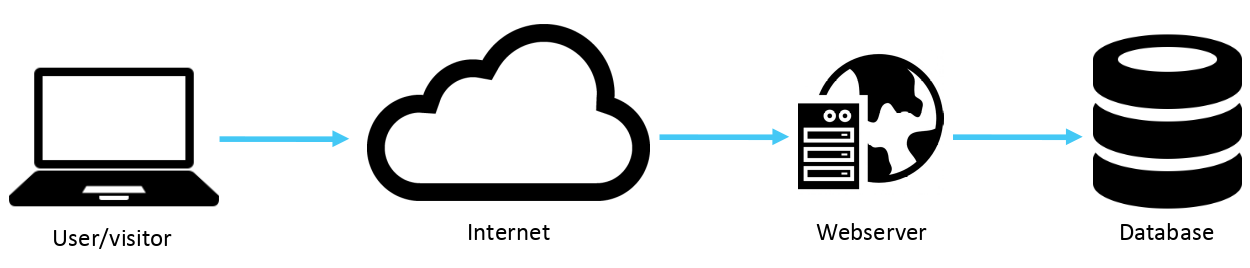
\includegraphics[width=0.5\textwidth]{loadbalancing1.png}
    \end{figure}
    \item Level 4 loadbalancing
    \begin{itemize}
        \item Simples form of loadbalancing
        \item IP+port combination
    \end{itemize}
    \begin{figure}[H]
        \centering
        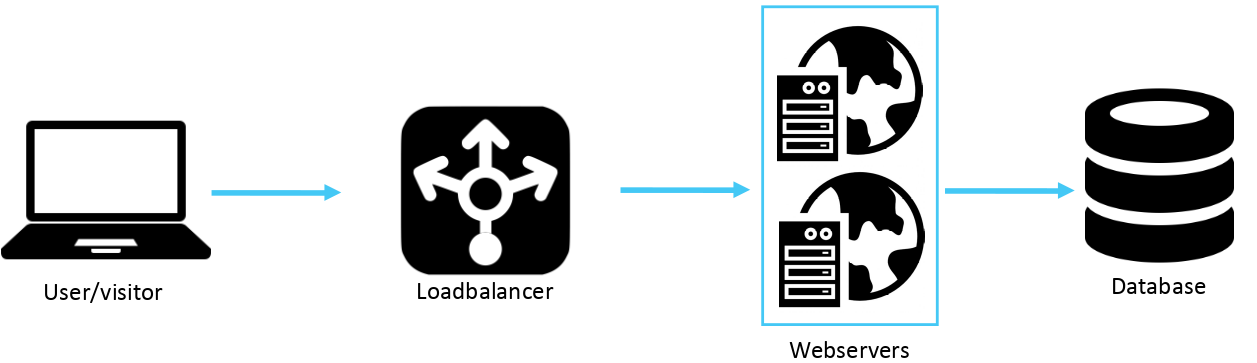
\includegraphics[width=0.5\textwidth]{loadbalancing2.png}
    \end{figure}
    \item Level 7 loadbalancing
    \begin{figure}[H]
        \centering
        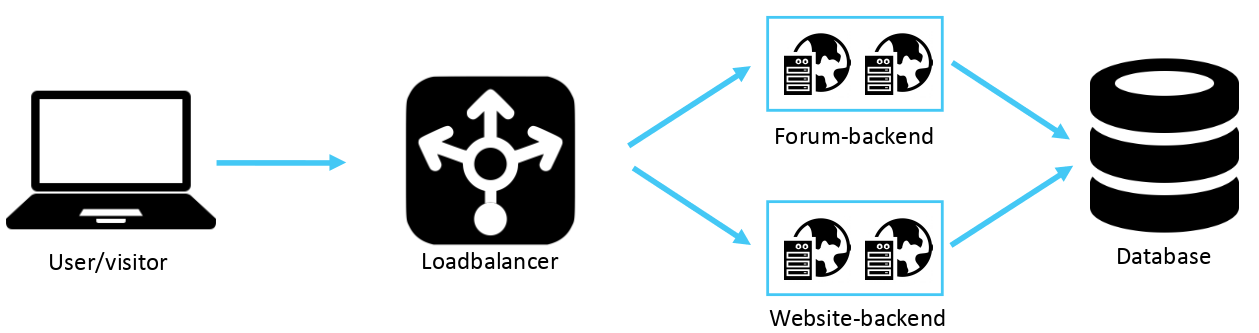
\includegraphics[width=0.5\textwidth]{loadbalancing3.png}
    \end{figure}
\end{itemize}




\subsection{HAProxy}

HAProxy is free, open-source software that provides a high availability load balancer
and proxy server for TCP and HTTP-based applications that spreads requests across multiple servers

Used by:

\begin{itemize}
    \item GitHub
    \item Imgur
    \item Instagram
    \item Twitter
    \item \dots
\end{itemize}

Configuration manual: \url{http://www.haproxy.org/download/2.0/doc/configuration.txt}

\subsubsection{Access Control Lists (ACLs)}

The ACLs test a certain condition, and link an action to that condition. Examples:

\begin{itemize}
    \item pattern matching (regex)
    \item number of connections
    \item \dots
\end{itemize}

\begin{minted}{bash}
# create an ACL that matches when the path of a request starts with /blog
# Example: http://yourdomain.com/blog/blog-entry-1
# the acl's name is url_blog
acl url_blog path_beg /blog
\end{minted}

You can send these actions to a backend

\subsubsection{Backend}

= Term for `the underlying web servers'

In our case: 2 webservers with apache httpd:

\begin{itemize}
    \item 192.168.X.20
    \item 192.168.X.30
\end{itemize}

Backend, in its simplest form, consists of:

\begin{itemize}
    \item Chosen loadbalancing algorithm
    \item List of webservers and portnumbers
\end{itemize}

Example configuration:

\begin{minted}{bash}
backend web-backend
    balance roundrobin
    server web1 web1.yourdomain.com:80 check
    server web2 web2.yourdomain.com:80 check

backend blog-backend
    balance roundrobin
    mode http
    server blog1 blog1.yourdomain.com:80 check
    server blog1 blog1.yourdomain.com:80 check
\end{minted}

\subsubsection{Frontend}

Specifies how requests should be forwarded to backends

\begin{itemize}
    \item Frontend consists in its simplest form of:
    \begin{itemize}
        \item Collection of IP addresses and port numbers
        \item ACLs
        \item `use\_backend' rules (determines which backend to use, based on ACLs)
    \end{itemize}
\end{itemize}

\subsubsection{Stickyness}

Some applications require that a user always connect to the same backend server.

\begin{itemize}
    \item This is called `sticky sessions'
    \item Parameter appsession in haproxy is used for this
\end{itemize}

\subsubsection{Health Checks}

\begin{itemize}
    \item Haproxy must know which backend server can handle all requests
    \item Simplest way: try 3-way open to the TCP port of each of the backend servers
    \item More advanced way: request web page of backend server, calculate hash, compare hash with hash of "OK" page
    \begin{itemize}
        \item Specific health check page that checks whether the application is still OK
    \end{itemize}
\end{itemize}

Server is alive $\Rightarrow$ is still participating in the load balancing

Server is dead? $\Rightarrow$ is automatically removed from load balancing

\subsubsection{High availability vs Load balancing}

High Availability

\begin{itemize}
    \item The goal is to \textbf{maximize availability}, usually by setting up different systems that can fulfill the same function
\end{itemize}

Load Balancing

\begin{itemize}
    \item The goal is to \textbf{distribute the load} between different systems that fulfill the same function
\end{itemize}

Combination of HA and LB is possible

\subsubsection{Installation haproxy}

\begin{minted}{bash}
# install the haproxy package
sudo apt install haproxy

# enable haproxy
sudo vim /etc/default/haproxy

# show haproxy version info
sudo haproxy -v
\end{minted}

\subsubsection{Configuration haproxy}

\begin{minted}{bash}
# this file contains configuration for frontend, backend and ACLs
sudo vim /etc/haproxy/haproxy.cfg
\end{minted}

\begin{minted}{bash}
frontend resume_site_front
    bind 192.168.X.10:80
    stats uri /haproxy?stats
    default_backend resume_site_back
 
 backend resume_site_back
    balance roundrobin
    server webserver1 192.168.X.20:80 check
    server webserver2 192.168.X.30:80 check
\end{minted}

\subsubsection{Start haproxy}

\begin{minted}{bash}
sudo systemctl restart haproxy
\end{minted}

Navigate to http://192.168.\textbf{X}.10/\textbf{haproxy?stats}

Security issues: do not enable this for remote connections (information disclosure)

\subsubsection{Check the operation of the loadbalancer}

\begin{enumerate}
    \item On both webservers: 
\begin{minted}{bash}
    # use this command to 'sniff' traffic
    tcpdump -flni any port 80
\end{minted}
    \item Browse to your public IP
\end{enumerate}

On both web servers, you can see some continuous movement

\begin{itemize}
    \item But we only requested our webpage once?
    \item This is because we do a check (see configuration) to check if the servers are alive
\end{itemize}

\subsubsection{General parameters}

httplog:

\begin{itemize}
    \item Enable logging of HTTP request, session state and timers
    \item By default: the log output format is very poor: it only contains the souce and destination addresses and the instance name
    \item By specifying `option httplog', each log line turns into a much richer format
\end{itemize}

httpclose:

\begin{itemize}
    \item Enable or disable passive HTTP connection closing
\end{itemize}

abortonclose:

\begin{itemize}
    \item Enable or disable early dropping of aborted requests pending in queues.
\end{itemize}

httpchk:

\begin{itemize}
    \item Enable HTTP protocol to check on the servers health
    \item Default: layer 4 health check
    \item `option httpchk' => layer 7 health check
    \item When "option httpchk" is specified, a complete HTTP request is sent once the TCP connection is established, 
        and responses 2xx and 3xx are considered valid, while all other ones indicate a server failure, 
        including the lack of any response.
\end{itemize}

\subsubsection{Health checks: parameters}

inter:

\begin{itemize}
    \item Interval (in seconds) between 2 consecutive health checks
    \item Default: 2 seconds
\end{itemize}

fastinter:

\begin{itemize}
    \item Interval (in seconds) between 2 consecutive health checks when state of backend server is `transitionally up' or `transitionally down'
    \item Default: value of inter
\end{itemize}

downinter:

\begin{itemize}
    \item Interval when backend server is down
    \item Default: value of inter
\end{itemize}

fall:

\begin{itemize}
    \item Number of consecutive failed health checks before a backend server gets status DOWN
    \item Default: 3
\end{itemize}

rise:

\begin{itemize}
    \item Number of consecutive succesful health checks before a backens server gets status UP
    \item Default: 2
\end{itemize}

\subsection{3 tips}

\subsubsection{Limit the number of simultaneous connections per host}

\begin{minted}{bash}
iptables -A INPUT -p tcp --syn --dport 80 -m connlimit --connlimit-above 15 
    --connlimit-mask 32 -j REJECT --reject-with tcp-reset
\end{minted}

\subsubsection{Transparent proxy with iptables and squid}

Iptables: forward to a squid proxy

\begin{minted}{bash}
iptables -t nat -A PREROUTING -i ens34 -s 192.168.45.0/24 
    -p tcp --dport 80 -j REDIRECT --to-port 3128

# Squid listens on 3128/TCP
\end{minted}

\subsubsection{Conntrack -L}

Conntrack = userspace tool to interact with kernelspace connection tracking module

\begin{minted}{bash}
# give a list of current connections being `tracked'
conntrack -L
\end{minted}



\end{document}